\documentclass[aspectratio=169,compress,12pt,dvipsnames]{beamer}

\usetheme{Arguelles}

%%%%%%%%%%%%%%%%%%%%%%%%%%%%%%%%%%%%%%%%%%%%%%%%%
%%%%%                                       %%%%%
%%%%%     LIST OF USEFUL LaTeX PACKAGES     %%%%%
%%%%%                                       %%%%%
%%%%%%%%%%%%%%%%%%%%%%%%%%%%%%%%%%%%%%%%%%%%%%%%%

% ---
% Character encoding
% ---
\usepackage[T1]{fontenc}
\usepackage[utf8]{inputenc}
\usepackage[]{fontawesome5}

% ---
% Language related packages
% ---
\usepackage[english]{babel}
\usepackage[abbreviations,british]{foreign}

% ---
% Bibliography-related
% ---
% \usepackage[numbers, sort&compress]{natbib}
%
% ---
% Colours
% ---
\usepackage[]{color}
\usepackage[]{xcolor}

% ---
% Figures
% ---
\usepackage[]{graphicx}
\usepackage[]{subfigure}

% ---
% Mathematics
% ---
\usepackage[]{mathtools}
\usepackage[]{amssymb, amsmath, amsfonts}
\usepackage[]{yhmath}
\usepackage[]{stmaryrd}
\usepackage[]{nicefrac}
\usepackage[]{algpseudocode}

% ---
% Physics
% ---
\usepackage[]{siunitx}
\usepackage[]{physics}

% ---
% Tikz-related
% ---
\usepackage[]{tikz}
\usetikzlibrary{arrows}
\usetikzlibrary{shapes}
\usetikzlibrary{positioning}
\usetikzlibrary{tikzmark}
\usetikzlibrary{patterns}
\usetikzlibrary{backgrounds}

% ---
% Miscellaneous
% ---
\usepackage[]{lipsum}
\usepackage[]{xparse}
\usepackage{multicol}

%%%%%%%%%%%%%%%%%%%%%%%%%%%%%%%%%%%%%%%%%%%%%%%
%%%%%                                     %%%%%
%%%%%     LIST OF COMMANDS AND MACROS     %%%%%
%%%%%                                     %%%%%
%%%%%%%%%%%%%%%%%%%%%%%%%%%%%%%%%%%%%%%%%%%%%%%

% ---
% Annotating equations using Tikz
% ---
\newcommand{\highlight}[2]{\colorbox{#1!17}{\ensuremath{\displaystyle #2}}}
\newcommand{\highlightdark}[2]{\colorbox{#1!47}{\ensuremath{\displaystyle #2}}}

% ---
% Mathematics
% ---

% Simple macros
\renewcommand{\det}[1]{\text{det}\left( #1 \right)}
\renewcommand{\trace}[1]{\text{Tr}\left( #1 \right)}
\newcommand{\Span}[1]{\text{Span}\left( #1 \right)}
\newcommand{\conj}[1]{\ensuremath{#1^*}}


% Algebra
\newcommand{\e}{\ensuremath{\mathrm{e}}}

\newcommand{\R}{\ensuremath{\mathbb{R}}}
\newcommand{\C}{\ensuremath{\mathbb{C}}}
\newcommand{\K}{\ensuremath{\mathbb{K}}}

\newcommand{\innerprod}[2]{\ensuremath{\left\langle #1 \vert #2 \right\rangle}}

% Linear algebra
\newcommand{\allones}{\ensuremath{\mathbf{1}}}
\newcommand{\allzeros}{\ensuremath{\mathbf{0}}}
\newcommand{\Gram}[1]{\ensuremath{\mathbf{#1}^T \mathbf{#1}}}
\newcommand{\inv}[1]{\ensuremath{\mathbf{#1}^{-1}}}
\newcommand{\pinv}[1]{\ensuremath{\mathbf{#1}^{\dagger}}}
\newcommand{\svd}[1]{\ensuremath{\mathbf{U}_{#1} \boldsymbol{\Sigma}_{#1} \mathbf{V}^T_{#1}}}

% Probability and statistics
\newcommand{\E}[1]{\ensuremath{\mathbb{E} \left[ #1 \right]}}
\newcommand{\covmat}[1]{\ensuremath{\mathbf{C}_{\mathbf{#1}}}}

% Optimization problems
\DeclareMathOperator*{\minimize}{minimize~}
\DeclareMathOperator*{\argmin}{argmin~}

\DeclareMathOperator*{\maximize}{maximize~}
\DeclareMathOperator*{\argmax}{argmax~}

\DeclareMathOperator{\subto}{subject~to~}

% Column and row vectors.
\ExplSyntaxOn
\NewDocumentCommand{\colvec}{O{1}m}
{
    \scalebox{#1}{$\generalvec{#2}{\\}$}
}
\NewDocumentCommand{\rowvec}{O{1}m}
{
    \scalebox{#1}{$\generalvec{#2}{&}$}
}
\NewDocumentCommand{\generalvec}{mm}
{
    \clist_set:Nn \l_tmpa_clist { #1 }
    %\renewcommand{\arraystretch}{.8}
    \begin{bmatrix}
        \clist_use:Nn \l_tmpa_clist { #2 }
    \end{bmatrix}
}
\ExplSyntaxOff
\usefonttheme{professionalfonts}

\graphicspath{{./imgs/}}

\title{Linear and nonlinear system identification}
\subtitle{Theoretical principles}
\event{CEA-EDF-INRIA Summer School}
\date{June 2025, EDF Lab Saclay}
\author{Jean-Christophe Loiseau}
%\institute{Arts \& Métiers}
\email{jean-christophe.loiseau@ensam.eu}
\homepage{loiseaujc.github.io}
%\github{loiseaujc}

\begin{document}

\frame[plain]{\titlepage}

%%%%%%%%%%%%%%%%%%%%%%%%%%%%%%%%
%%%%%     INTRODUCTION     %%%%%
%%%%%%%%%%%%%%%%%%%%%%%%%%%%%%%%

\begin{frame}
    \vfill
    \begin{minipage}{.28\textwidth}
        \centering
        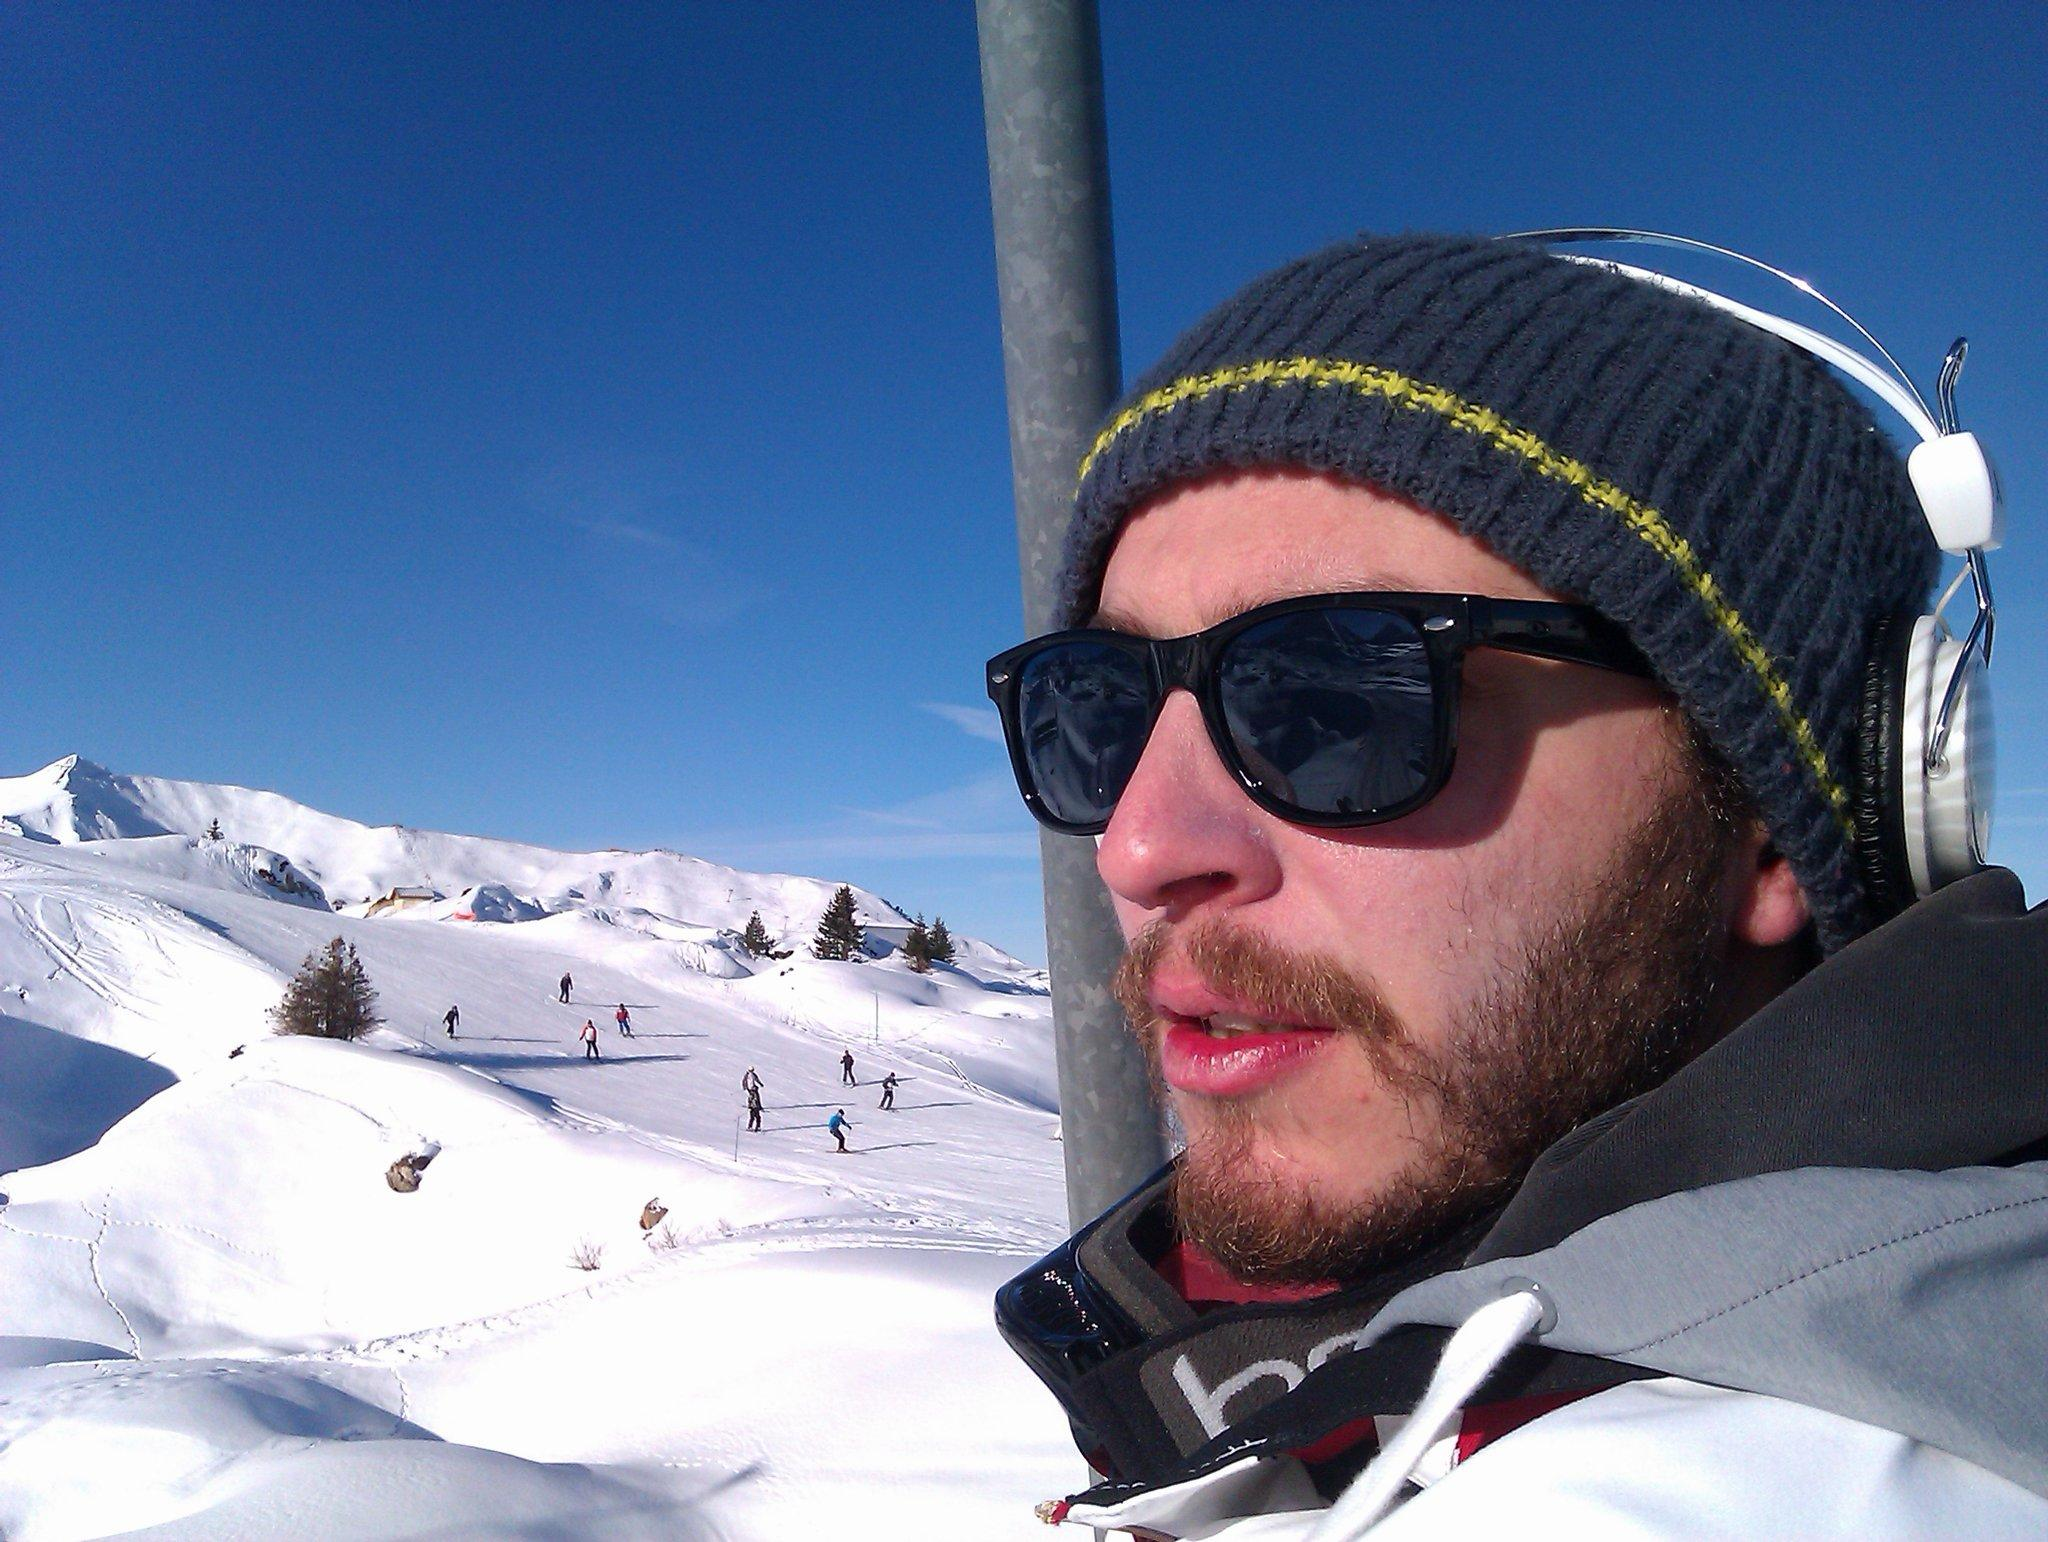
\includegraphics[width=\textwidth]{myself.jpg}  \\
        \par\bigskip
        \tiny
        Assistant Professor of Applied Mathematics and Fluid Dynamics
    \end{minipage}%
    \hfill
    \begin{minipage}{.68\textwidth}
        \centering
        \begin{tabular}{rl}
            \textbf{Research activities}    &   Hydrodynamic instabilities  \\
                                            &   Transition to turbulence    \\
                                            &   Reduced-order modeling      \\
                                            &   Optimal control             \\
                                                                            \\
            \textbf{Tools}                  &   High-performance computing  \\
                                            &   Numerical Linear Algebra    \\
                                            &   Convex optimization
        \end{tabular}
    \end{minipage}
    \vfill
\end{frame}

\begin{frame}[t, c]{Non-exhaustive list of challenges}
    \vfill
    \begin{minipage}{.68\textwidth}
        \centering
        \begin{tabular}{rl}
            \textbf{Physics}    &   What is physically realizable?      \\
                                &   What are the operating conditions?  \\
                                &   Which mechanisms to leverage?       \\
                                &   How to identify them?               \\
                                &   How generic are they?
        \end{tabular}
    \end{minipage}%
    \hfill
    \begin{minipage}{.28\textwidth}
        \centering
        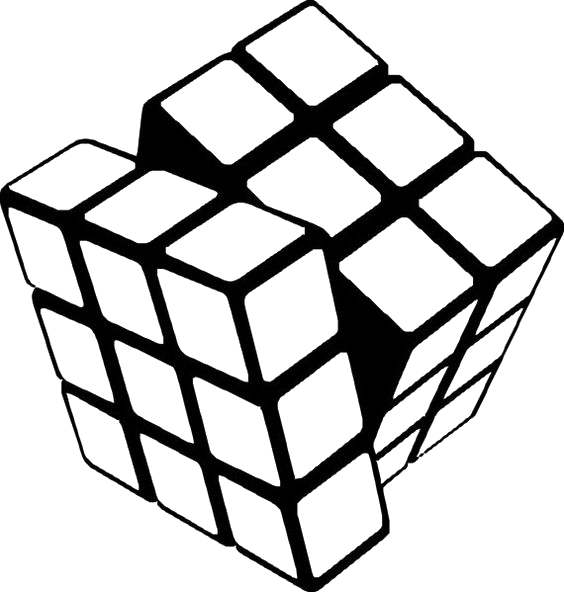
\includegraphics[width=\textwidth]{rubik_cube.png}
    \end{minipage}
    \vfill
\end{frame}


\begin{frame}[t, c]{Non-exhaustive list of challenges}
    \vfill
    \begin{minipage}{.68\textwidth}
        \centering
        \begin{tabular}{rl}
            \textbf{Instrumentation}    &   What is actually \emph{observable}? \\
                                        &   What kind of sensors can I use?     \\
                                        &   Where to place them and how many?   \\
                                        &   How to handle measurement noise?    \\
                                        &   What if one of my sensor fail?
        \end{tabular}
    \end{minipage}%
    \hfill
    \begin{minipage}{.28\textwidth}
        \centering
        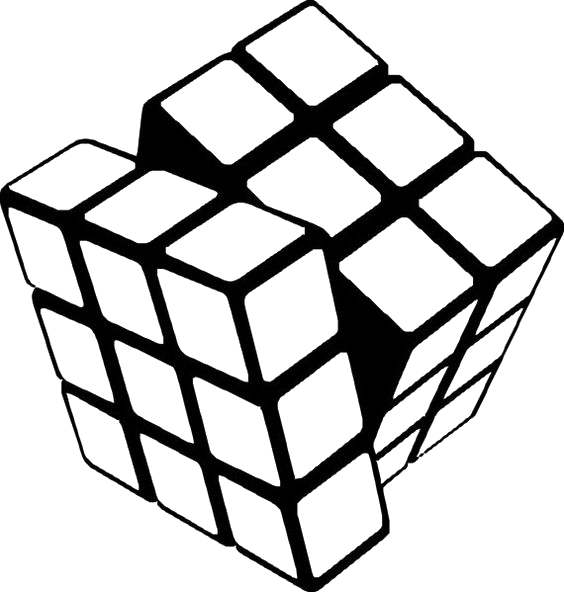
\includegraphics[width=\textwidth]{rubik_cube.png}
    \end{minipage}
    \vfill
\end{frame}

\begin{frame}[t, c]{Non-exhaustive list of challenges}
    \vfill
    \begin{minipage}{.68\textwidth}
        \centering
        \begin{tabular}{rl}
            \textbf{Instrumentation}    &   What is actually \emph{controllable}?   \\
                                        &   What kind of actuators can I use?       \\
                                        &   Where to place them and how many?       \\
                                        &   How to handle disturbances?             \\
                                        &   What if one of my actuator fail?
        \end{tabular}
    \end{minipage}%
    \hfill
    \begin{minipage}{.28\textwidth}
        \centering
        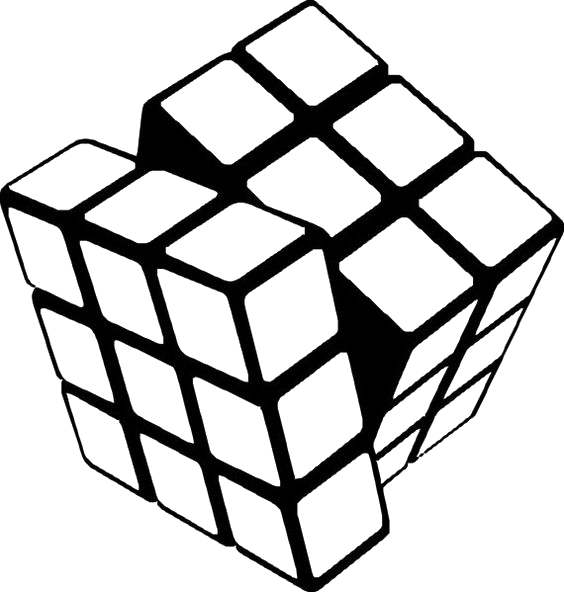
\includegraphics[width=\textwidth]{rubik_cube.png}
    \end{minipage}
    \vfill
\end{frame}

\begin{frame}[t, c]{Non-exhaustive list of challenges}
    \vfill
    \begin{minipage}{.68\textwidth}
        \centering
        \begin{tabular}{rl}
            \textbf{Control}    &   What are the specifications?            \\
                                &   How robust does it need to be?          \\
                                &   Do I have hard operating constraints?   \\
                                &   On-board or external computations?      \\
                                &   Do I need any form of certification?
        \end{tabular}
    \end{minipage}%
    \hfill
    \begin{minipage}{.28\textwidth}
        \centering
        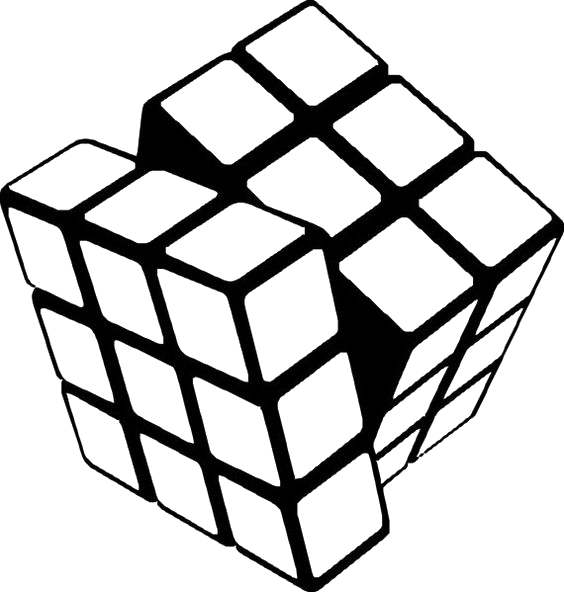
\includegraphics[width=\textwidth]{rubik_cube.png}
    \end{minipage}
    \vfill
\end{frame}

\begin{frame}[t, c]{Non-exhaustive list of challenges}
    \vfill
    \begin{minipage}{.68\textwidth}
        \centering
        \begin{tabular}{rl}
            \textbf{Modelling}  &   What kind of model?                 \\
                                &   Physics-based or data-driven?       \\
                                &   How accurate does it need to be?    \\
                                &   Can I quantify the uncertainties?   \\
                                &   How expensive is it simulate?
        \end{tabular}
    \end{minipage}%
    \hfill
    \begin{minipage}{.28\textwidth}
        \centering
        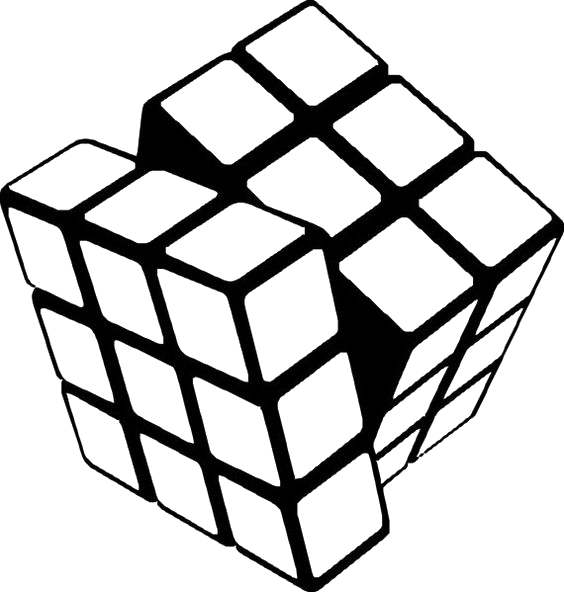
\includegraphics[width=\textwidth]{rubik_cube.png}
    \end{minipage}
    \vfill
\end{frame}

\section{Linear System Identification}

\begin{frame}[standout, plain]
    \usebeamerfont{title}
    Linear System Identification

    \usebeamerfont{subtitle}
    A brief overview
\end{frame}

\begin{frame}
    \vfill
    \[
        \begin{aligned}
            \vb{x}_{t+1} & = \vb{A} \vb{x}_t + \vb{B} \tikzmarknode{a}{\highlightdark{blue}{\vb{u}}}_t\\
            \tikzmarknode{b}{\highlightdark{Green}{\vb{y}}}_{t} & = \vb{C} \vb{x}_t + \vb{D} \vb{u}_t.
        \end{aligned}
    \]
    \begin{tikzpicture}[overlay, remember picture, >=stealth, nodes={align=left, inner ysep=1pt}, <-]
        \path (a.north) ++ (0, 1em) node[anchor=south west, color=blue!67] (dynamics){Known input sequence};
        \draw [color=blue!87] (a.north) |- ([xshift=0.3ex, color=blue] dynamics.south east);

        \path (b.south) ++ (0, -1em) node[anchor=north east, color=Green!67] (actuators){Measured output sequence};
        \draw [color=Green!87] (b.south) |- ([xshift=0.3ex, color=Green] actuators.south west);
    \end{tikzpicture}
    \vfill
\end{frame}

\begin{frame}
    \vfill
    \centering
    \underline{\textbf{Kalman decomposition}}

    \begin{overprint}
        \onslide<1>
        \[
            \begin{aligned}
                \colvec{\vb{x}_{r\overline{o}}, \vb{x}_{ro}, \vb{x}_{\overline{ro}}, \vb{x}_{\overline{r}o}}_{t+1}
                &   =
                \begin{bmatrix}
                    \vb{A}_{r\overline{o}}  &   * &   * &   * \\
                    &   \vb{A}_{ro} &   *   &   * \\
                    &               &   \vb{A}_{\overline{ro}}  &   * \\
                    &               &                           &   \vb{A}_{\overline{r}o}
                \end{bmatrix}
                \colvec{\vb{x}_{r\overline{o}}, \vb{x}_{ro}, \vb{x}_{\overline{ro}}, \vb{x}_{\overline{r}o}}_{t}
                +
                \colvec{\vb{B}_{r\overline{o}}, \vb{B}_{ro}, \allzeros, \allzeros} \vb{u}_t \\
                %
                \vb{y}_t    &   =   \rowvec{\allzeros, \vb{C}_{ro}, \allzeros, \vb{C}_{\overline{r}o}}
                \colvec{\vb{x}_{r\overline{o}}, \vb{x}_{ro}, \vb{x}_{\overline{ro}}, \vb{x}_{\overline{r}o}}_{t}    +   \vb{Du}_t
            \end{aligned}
        \]
        \onslide<2>
        \[
            \begin{aligned}
                \colvec{\vb{x}_{r\overline{o}}, \vb{x}_{ro}, \vb{x}_{\overline{ro}}, \vb{x}_{\overline{r}o}}_{t+1}
                &   =
                \begin{bmatrix}
                    \vb{A}_{r\overline{o}}  &   * &   * &   * \\
                    &   \highlightdark{blue}{\vb{A}_{ro}} &   *   &   * \\
                    &               &   \vb{A}_{\overline{ro}}  &   * \\
                    &               &                           &   \vb{A}_{\overline{r}o}
                \end{bmatrix}
                \colvec{\vb{x}_{r\overline{o}}, \vb{x}_{ro}, \vb{x}_{\overline{ro}}, \vb{x}_{\overline{r}o}}_{t}
                +
                \colvec{\vb{B}_{r\overline{o}}, \highlightdark{blue}{\vb{B}_{ro}}, \allzeros, \allzeros} \vb{u}_t \\
                %
                \vb{y}_t    &   =   \rowvec{\allzeros, \highlightdark{blue}{\vb{C}_{ro}}, \allzeros, \vb{C}_{\overline{r}o}}
                \colvec{\vb{x}_{r\overline{o}}, \vb{x}_{ro}, \vb{x}_{\overline{ro}}, \vb{x}_{\overline{r}o}}_{t}    +   \highlightdark{blue}{\vb{D}}\vb{u}_t
            \end{aligned}
        \]
        %
        In practice, only a realization of the jointly observable and controllable subsystem $(\vb{A}_{ro}, \vb{B}_{ro}, \vb{C}_{ro}, \vb{D})$ can be obtained from data.
    \end{overprint}
    \vfill
\end{frame}

\begin{frame}
    \vfill
    The realization of the jointly controllable and observable subsystem is not unique.
    \vfill
    \begin{minipage}{.48\textwidth}
        \[
            \begin{aligned}
                \vb{x}_{t+1} & = \vb{Ax}_t + \vb{Bu}_t \\
                \vb{y}_t & = \vb{Cx}_t + \vb{Du}_t
            \end{aligned}
        \]
    \end{minipage}%
    \hfill
    \begin{minipage}{.48\textwidth}
        \[
            \begin{aligned}
                \vb{z}_{t+1} & = \vb{T}^{-1} \vb{ATz}_t + \vb{T}^{-1}\vb{Bu}_t \\
                \vb{y}_t & = \vb{CTz}_t + \vb{Du}_t
            \end{aligned}
        \]
    \end{minipage}
    \vfill
    Both models have the same I/O behavior and are thus equivalent representations of the same system.
    \vfill
\end{frame}

\begin{frame}[standout, plain]
    \usebeamerfont{title}
    Linear System Identification

    \usebeamerfont{subtitle}
    Realization theory
\end{frame}

\begin{frame}
    \vfill
    \[
        \begin{aligned}
            \vb{x}_{t+1} & = \vb{A} \vb{x}_t + \vb{B} \tikzmarknode{a}{\highlightdark{blue}{\vb{u}}}_t\\
            \tikzmarknode{b}{\highlightdark{Green}{\vb{y}}}_{t} & = \vb{C} \vb{x}_t + \vb{D} \vb{u}_t.
        \end{aligned}
    \]
    \begin{tikzpicture}[overlay, remember picture, >=stealth, nodes={align=left, inner ysep=1pt}, <-]
        \path (a.north) ++ (0, 1em) node[anchor=south west, color=blue!67] (dynamics){Known input sequence};
        \draw [color=blue!87] (a.north) |- ([xshift=0.3ex, color=blue] dynamics.south east);

        \path (b.south) ++ (0, -1em) node[anchor=north east, color=Green!67] (actuators){Measured output sequence};
        \draw [color=Green!87] (b.south) |- ([xshift=0.3ex, color=Green] actuators.south west);
    \end{tikzpicture}
    \vfill
\end{frame}

\begin{frame}
    \vfill
    Given the (yet unknown) states at time $t=1$ and $t=2$, we can write
    \[
        \vb{x}_2  = \vb{Ax}_1 + \vb{B}\vb{u}_1, \quad \vb{x}_3  = \vb{Ax}_2 + \vb{B}\vb{u}_2, \quad \vb{x}_4  = \vb{Ax}_3 + \vb{B}\vb{u}_3,
    \]
    %
    or alternatively
    %
    \[
        \vb{x}_3 = \vb{A}^2\vb{x}_1 + \vb{A}\vb{B}\vb{u}_1 + \vb{B}\vb{u}_2, \quad \vb{x}_4 = \vb{A}^2 \vb{x}_2 + \vb{A}\vb{B}\vb{u}_2 + \vb{B}\vb{u}_3
    \]
    %
    leading to
    %
    \[
        \rowvec{\vb{x}_3, \vb{x}_4}  = \vb{A}^2 \rowvec{\vb{x}_1, \vb{x}_2} + \rowvec{\vb{A}\vb{B}, \vb{B}} \begin{bmatrix} \vb{u}_1 & \vb{u}_2 \\ \vb{u}_2 & \vb{u}_3 \end{bmatrix}.
    \]
    \vfill
\end{frame}

\begin{frame}
    \vfill
    \[
        \begin{bmatrix}
            \vb{y}_k & \vb{y}_{k+1} \\ \vb{y}_{k+1} & \vb{y}_{k+2}
        \end{bmatrix}
        =
        \colvec{\vb{C}, \vb{CA}}
        \rowvec{\vb{x}_k, \vb{x}_{k+1}}
        +
        \begin{bmatrix}
            \vb{D} \\ \vb{CB} & \vb{D}
        \end{bmatrix}
        \begin{bmatrix}
            \vb{u}_k & \vb{u}_{k+1} \\ \vb{u}_{k+1} & \vb{u}_{k+2}
        \end{bmatrix}
    \]
    %
    \vfill
    %
    \begin{minipage}{.48\textwidth}
        \centering
        \underline{Past data}
        %
        \[
            \vb{X}_p = \mathcal{O}^{\dagger} \left( \vb{Y}_p - \vb{HU}_p \right)
        \]
    \end{minipage}%
    \hfill
    \begin{minipage}{.48\textwidth}
        \centering
        \underline{Future data}
        %
        \[
            \mathcal{O} \vb{X}_f = \vb{Y}_f - \vb{HU}_f
        \]
    \end{minipage}
    \vfill
\end{frame}

\begin{frame}
    \vfill
    \[
        \tikzmarknode{a}{\highlightdark{red}{\vb{Y}_f}} - \vb{H} \tikzmarknode{b}{\highlightdark{blue}{\vb{U}_f}} = \mathcal{O} \vb{A}^k \mathcal{O}^{\dagger} \tikzmarknode{c}{\highlightdark{Green}{\vb{Y}_p}} + \mathcal{O} \left( \boldsymbol{\Delta} - \vb{A}^k \mathcal{O}^{\dagger} \vb{H} \right) \tikzmarknode{d}{\highlightdark{Plum}{\vb{U}_p}}
    \]
    \begin{tikzpicture}[overlay, remember picture, >=stealth, nodes={align=left, inner ysep=1pt}, <-]
        \path (a.north) ++ (0, 2em) node[anchor=south west, color=red!67] (yf){Future output};
        \draw [color=red!87] (a.north) |- ([xshift=0.3ex, color=red] yf.south east);

        \path (b.south) ++ (0, -2em) node[anchor=north east, color=blue!67] (uf){Future input};
        \draw [color=blue!87] (b.south) |- ([xshift=0.3ex, color=blue] uf.south west);

        \path (c.north) ++ (0, 2em) node[anchor=south west, color=Green!67] (yp){Past output};
        \draw [color=Green!87] (c.north) |- ([xshift=0.3ex, color=Green] yp.south east);

        \path (d.south) ++ (0, -2em) node[anchor=north east, color=Plum!67] (up){Past input};
        \draw [color=Plum!87] (d.south) |- ([xshift=0.3ex, color=Plum] up.south west);    
    \end{tikzpicture}
    \vfill
\end{frame}

\begin{frame}
    \vfill
    \begin{minipage}{.38\textwidth}
        \[
            \mathcal{O}
            =
            \colvec{\vb{C}, \vb{CA}, \vb{CA}^2, \vdots, \vb{CA}^{k-1}}
        \]

        \[
            \boldsymbol{\Delta}
            =
            \rowvec{\vb{A}^{k-1} \vb{B}, \vb{A}^{k-2} \vb{B}, \cdots, \vb{AB}, \vb{B}}
        \]
    \end{minipage}%
    \hfill
    \begin{minipage}{.58\textwidth}
        \[
            \vb{H}
            =
            \begin{bmatrix}
                \vb{D}  \\
                \vb{CB} &   \vb{D}  \\
                \vb{CAB}    &   \vb{CB} &   \vb{D}  \\
                \vb{CA}^2 \vb{B}    &   \vb{CAB}    &   \vb{CB} &   \vb{D}  \\
                \vdots  &   \ddots  &   \ddots      &   \ddots  &   \ddots  \\
                \vb{CA}^{k-1}\vb{B} &   \vb{CA}^{k-2}\vb{B} & \cdots & \vb{CAB} & \vb{CB} & \vb{D}
            \end{bmatrix}
        \]
    \end{minipage}
    \vfill
\end{frame}

\begin{frame}
    \vfill
    The problem we'd like to solve reads
    \[
        \minimize \quad \norm{\vb{Y}_f - \vb{H} \vb{U}_f - \mathcal{O} \vb{A}^k \mathcal{O}^{\dagger} \vb{Y}_p + \mathcal{O} \left( \boldsymbol{\Delta} - \vb{A}^k \mathcal{O}^{\dagger} \vb{H} \right) \vb{U}_p}_F^2
    \]
    %
    It however is a non-convex problem.
    \vfill
\end{frame}

\begin{frame}
    \vfill
    Let $\vb{W} = \vb{I} - \vb{U}_f^T \left( \vb{U}_f \vb{U}_f^T \right)^{-1} \vb{U}_f$ and $k$ large enough, the problem reduces to
    %
    \[
        \begin{aligned}
            \minimize   &   \norm{\vb{M}^{\frac12} \left( \vb{Y}_f - \mathcal{O}\boldsymbol{\Delta} \vb{U}_p \right) \vb{W}^{\frac12}}_F^2  \\
            \subto      &   \rank(\mathcal{O}\boldsymbol{\Delta}) = r
        \end{aligned}
    \]
    %
    which can be cast as a \emph{Quadratic Program with Quadratic equality constraints} admitting a closed-form solution.
    \vfill
\end{frame}

\begin{frame}
    \vfill
    \centering
    \[
        \begin{aligned}
            \minimize_{\mathcal{O}, \boldsymbol{\Delta}} & \quad \dfrac12 \trace{\boldsymbol{\Delta}^T \vb{U}_p^T \vb{WU}_p \boldsymbol{\Delta}} - \trace{\mathcal{O}^T \vb{M} \vb{Y}_f^T \vb{WU}_p \boldsymbol{\Delta}} \\
            \subto & \quad \mathcal{O}^T \vb{M} \mathcal{O} = \vb{I}_r
        \end{aligned}
    \]
    
    \vfill

    \underline{\textbf{Quadratic Program with Quadratic Equality constraints}}
    \vfill
\end{frame}

\begin{frame}
    \vfill
    \centering
    \[
        \begin{aligned}
            \minimize_{\mathcal{O}, \boldsymbol{\Delta}} & \quad \trace{\rowvec{\mathcal{O}^T, \boldsymbol{\Delta}^T} \begin{bmatrix} \allzeros & -\mathbf{MY}_f \mathbf{WU}_p \\ -\mathbf{U}_p^T \mathbf{WY}_f \vb{M} & \mathbf{U}_p \mathbf{WU}_p \end{bmatrix} \colvec{\mathcal{O}, \boldsymbol{\Delta}}} \\
            %
            \subto & \rowvec{\mathcal{O}^T, \boldsymbol{\Delta}^T} \begin{bmatrix} \vb{M} & \allzeros \\ \allzeros & \allzeros \end{bmatrix} \colvec{\mathcal{O}, \boldsymbol{\Delta}} = \vb{I}_r
        \end{aligned}
    \]

    \vfill

    \underline{\textbf{Trace minimization of a Hermitian matrix}}

    \vfill
\end{frame}

\begin{frame}
    \vfill
    \centering
    \[
        \begin{bmatrix}
            \vb{M} & \allzeros \\
            \allzeros & \allzeros
        \end{bmatrix}
        \colvec{\mathcal{O}, \boldsymbol{\Delta}}
        \boldsymbol{\Lambda}
        =
        \begin{bmatrix}
            \allzeros & -\vb{MY}_f \vb{WU}_p \\
            - \vb{U}_p^T \vb{WY}_f \vb{M} & \vb{U}_p \vb{WU}_p
        \end{bmatrix}
        \colvec{\mathcal{O}, \boldsymbol{\Delta}}
    \]
    \vfill
    \underline{\textbf{Generalized eigenvalue problem}}
    \vfill
\end{frame}

\begin{frame}
    \vfill
    \centering
    \begin{tabular}{cccc}
        &   N4SID   &   MOESP   &   CVA \\
        \hline
        $\vb{M}$    &   $\vb{I}$    &   $\vb{I}$    &   $\left( \vb{Y}_f \boldsymbol{\Pi}_{\vb{U}}^{\perp} \vb{Y}_f^T \right)^{-1}$ \\
        $\vb{W}$    &   ?           &   $\boldsymbol{\Pi}_{\vb{U}^{\perp}}$   &   $\boldsymbol{\Pi}_{\vb{U}}^{\perp}$ 
    \end{tabular}
    \vfill
\end{frame}

\begin{frame}
    \vfill
    \centering
    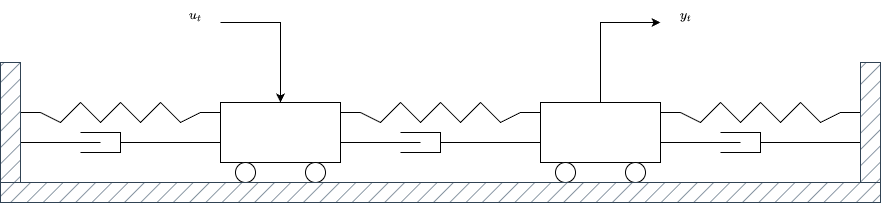
\includegraphics[width=.8\textwidth]{mechanical_system.png}
    \vfill
\end{frame}

\begin{frame}
    \vfill
    \centering
    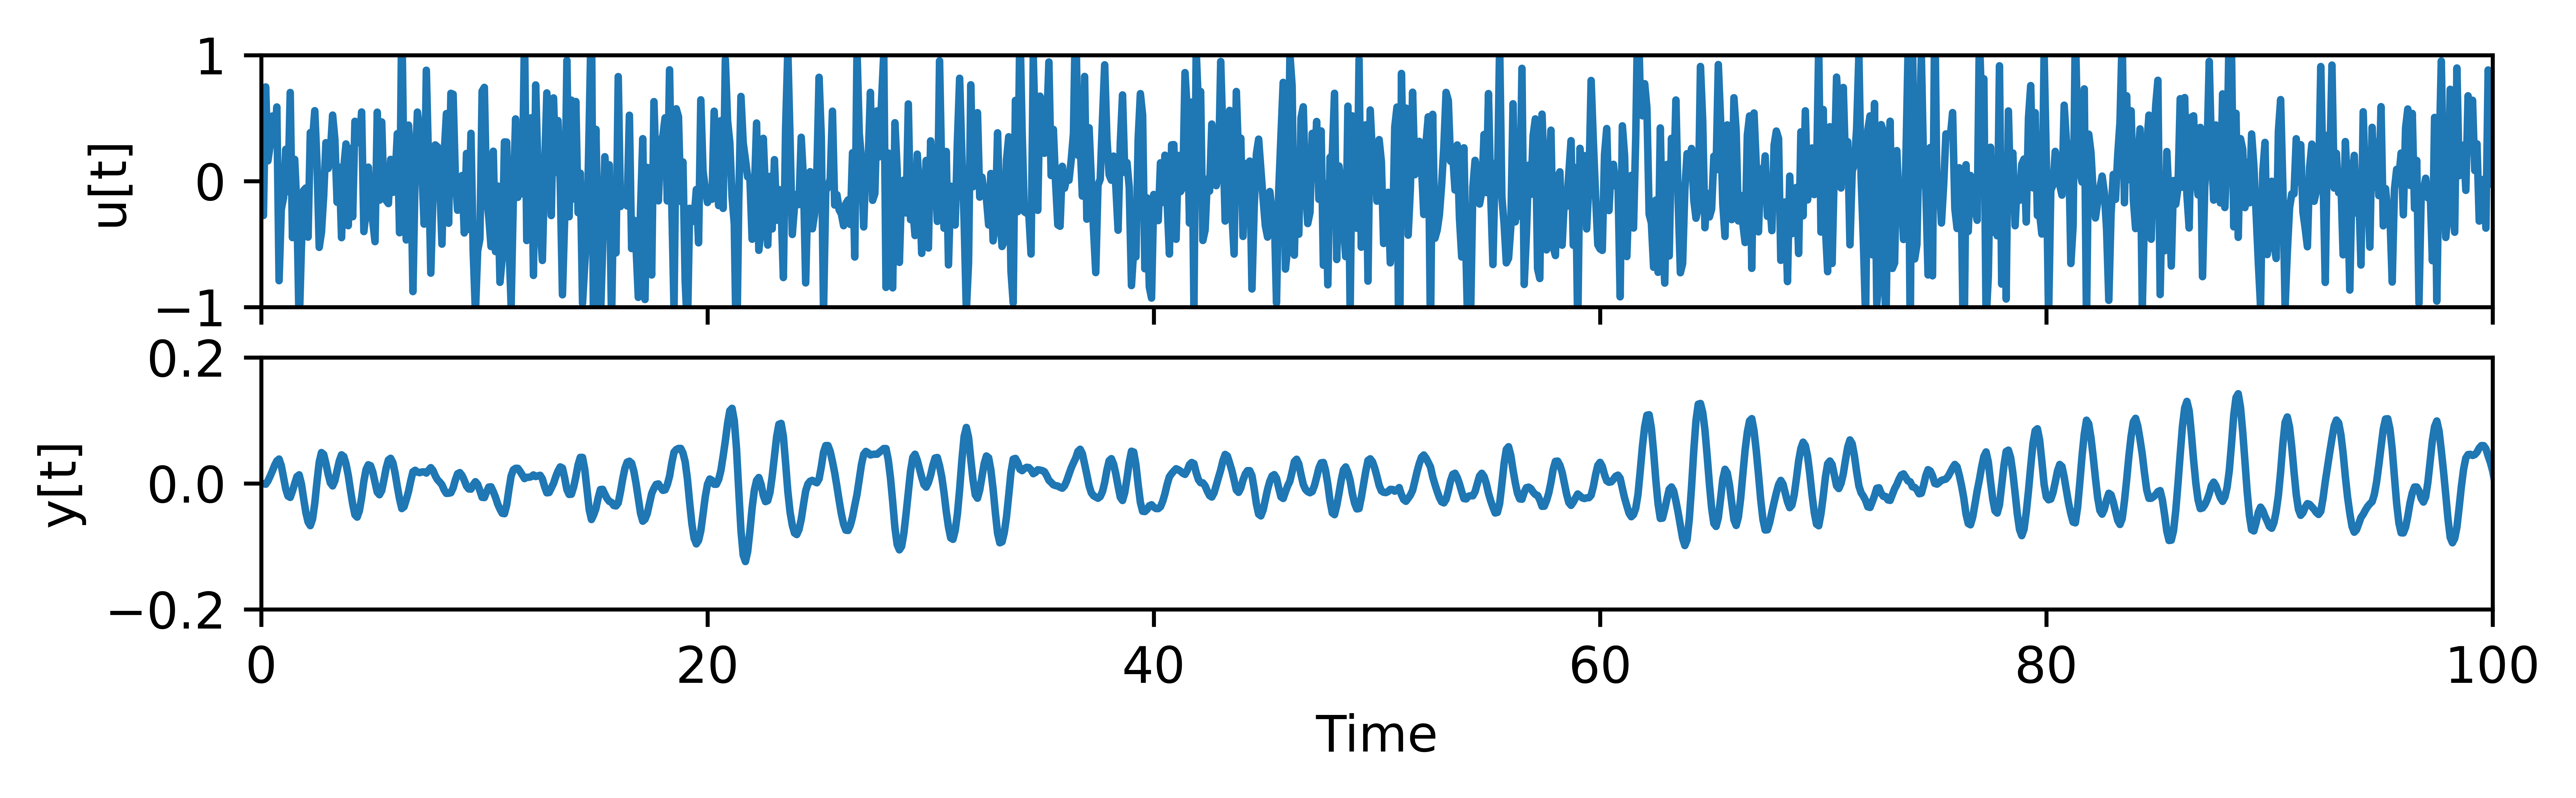
\includegraphics[width=.8\textwidth]{io_data.png}
    \vfill
\end{frame}

\begin{frame}
    \vfill
    \begin{minipage}{.68\textwidth}
        \[
            \vb{A}
            =
            \begin{bmatrix}
                0.95 & -0.28 & -0.01 & 0.03 \\
                0.28 & 0.95 & -0.03 & 0.005 \\
                -0.007 & 0.017 & 0.84 & 0.52 \\
                -0.01 & 0.002 & -0.49 & 0.84
            \end{bmatrix}
        \]
        \bigskip
        \[
            \vb{B} = \colvec{0.054, -0.03, 0.05, 0.03}, \quad \vb{C} = \rowvec{0.1, 0.07, 0.2, -0.12}
        \]
    \end{minipage}%
    \hfill
    \begin{minipage}{.28\textwidth}
        \centering
        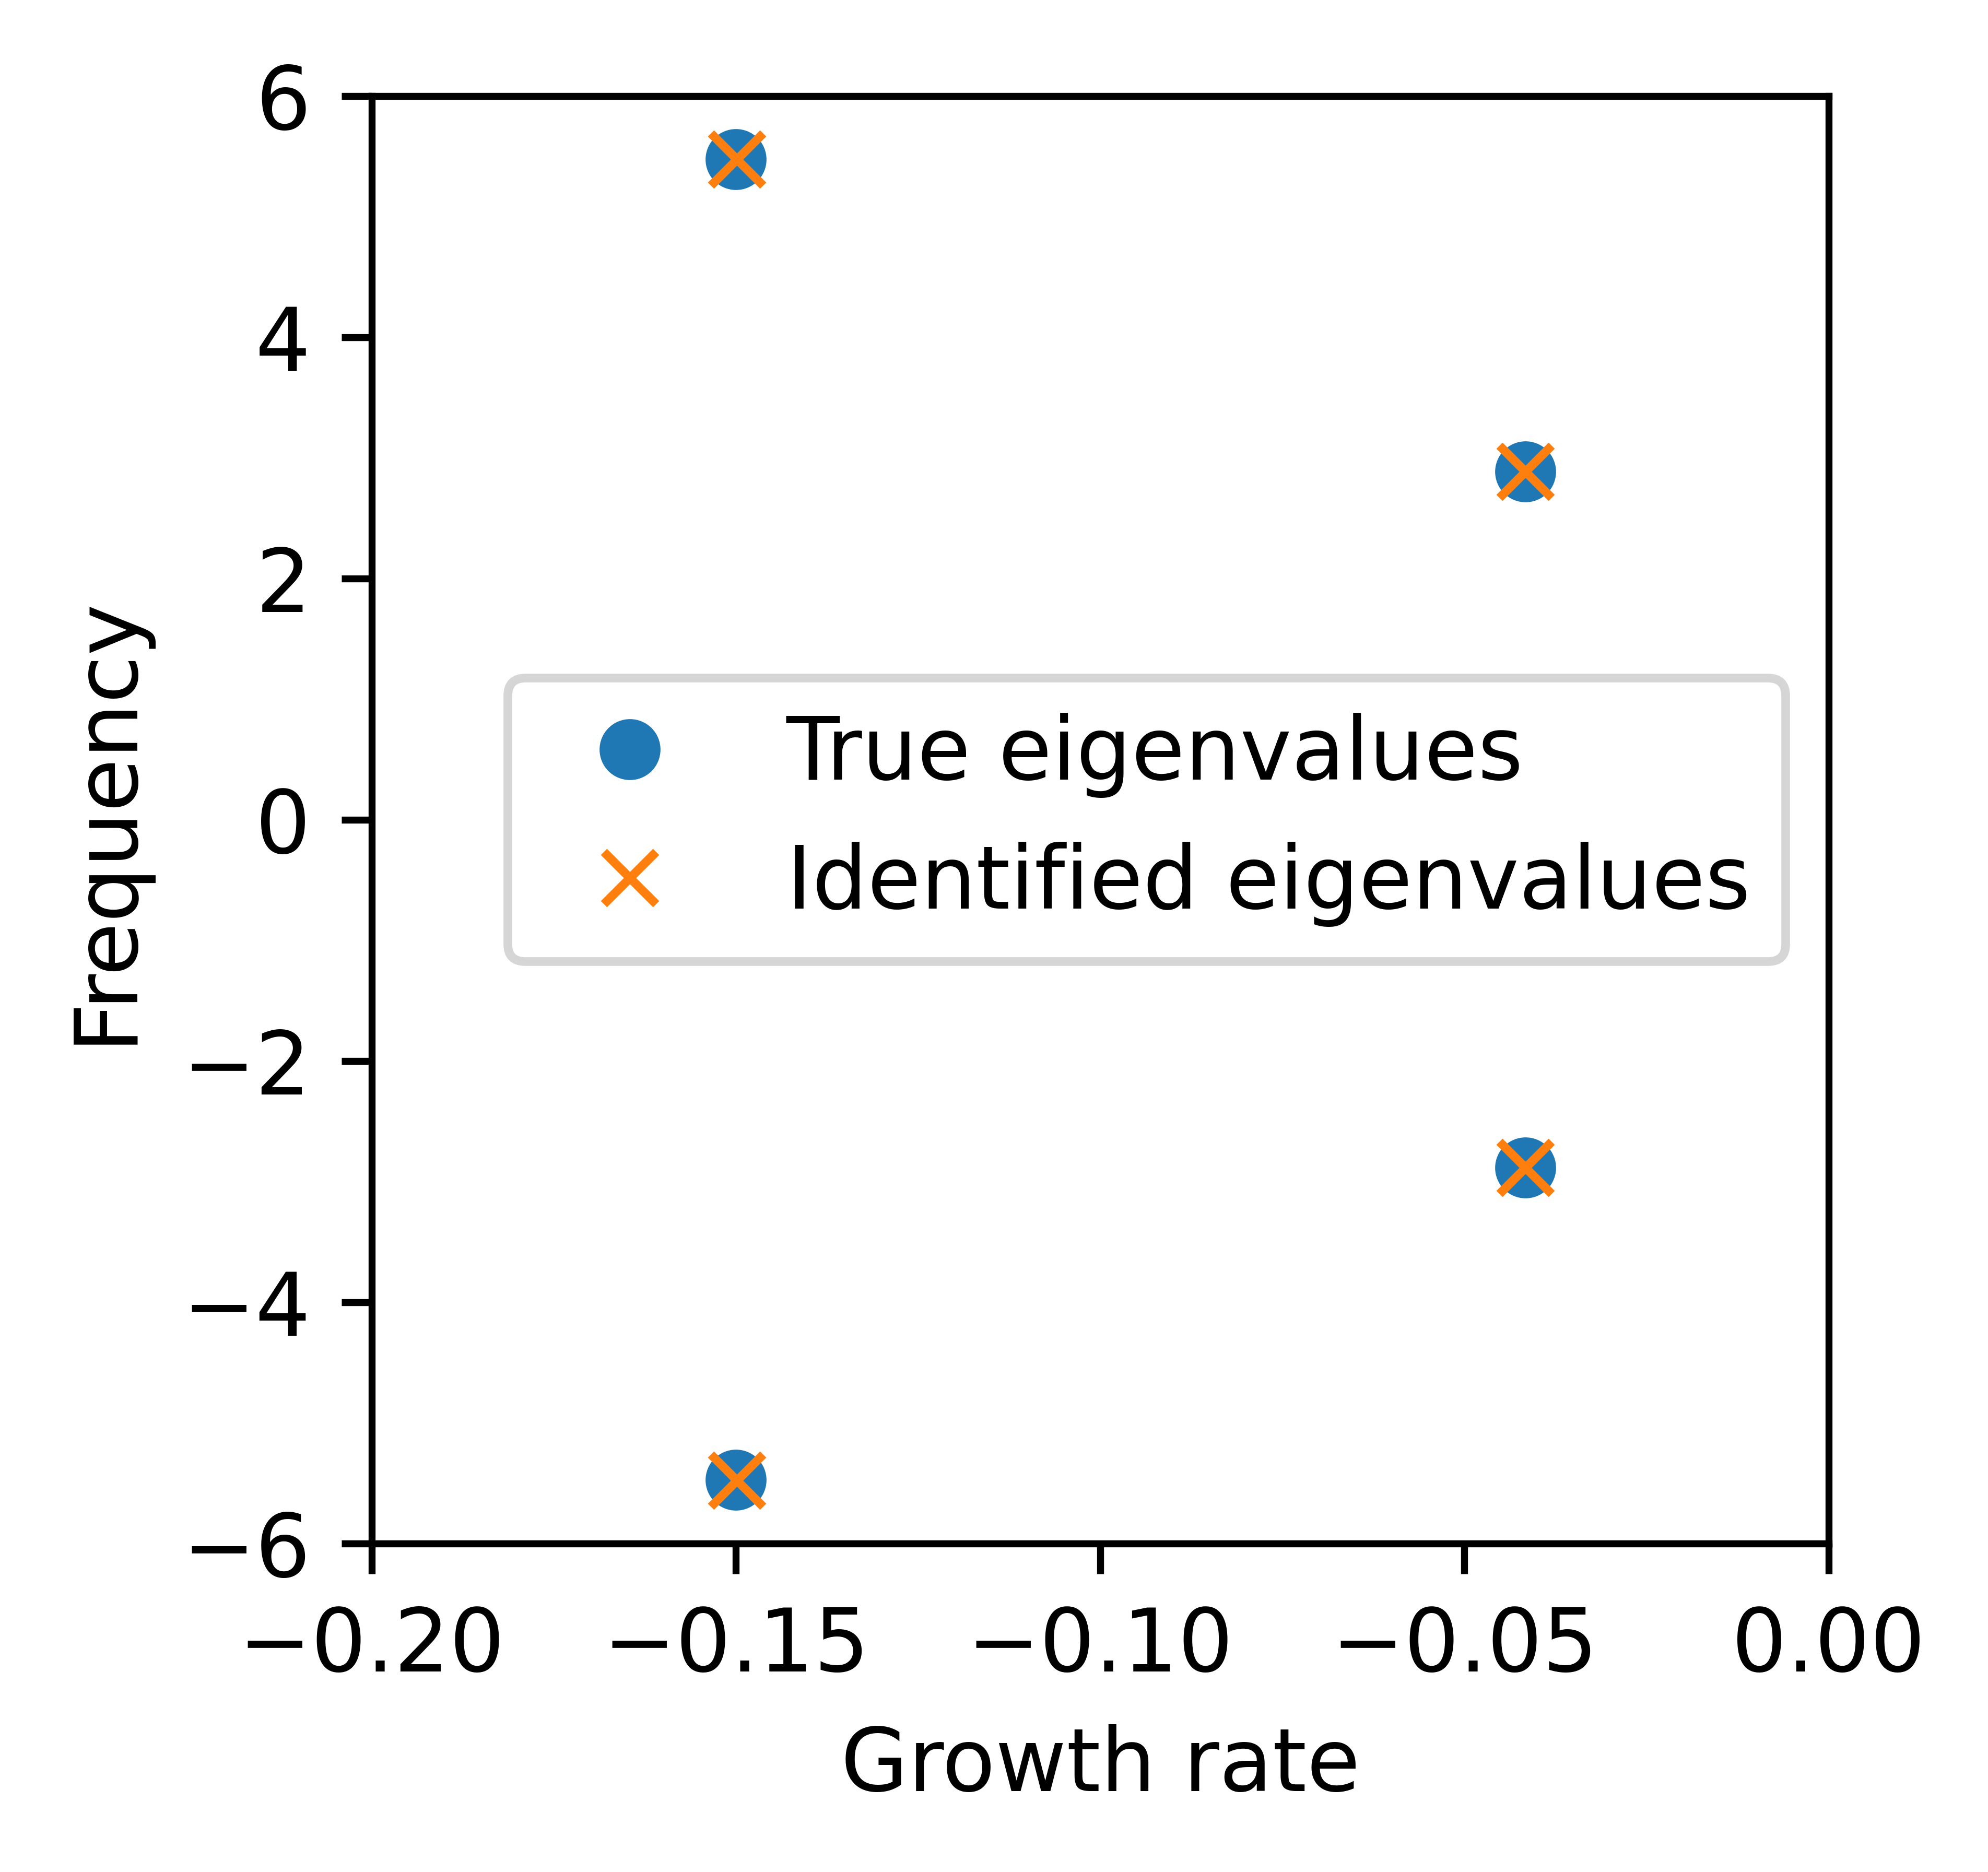
\includegraphics[width=\textwidth]{identified_eigenspectrum.png}
    \end{minipage}
    \vfill
\end{frame}

\begin{frame}
    \vfill
    \centering
    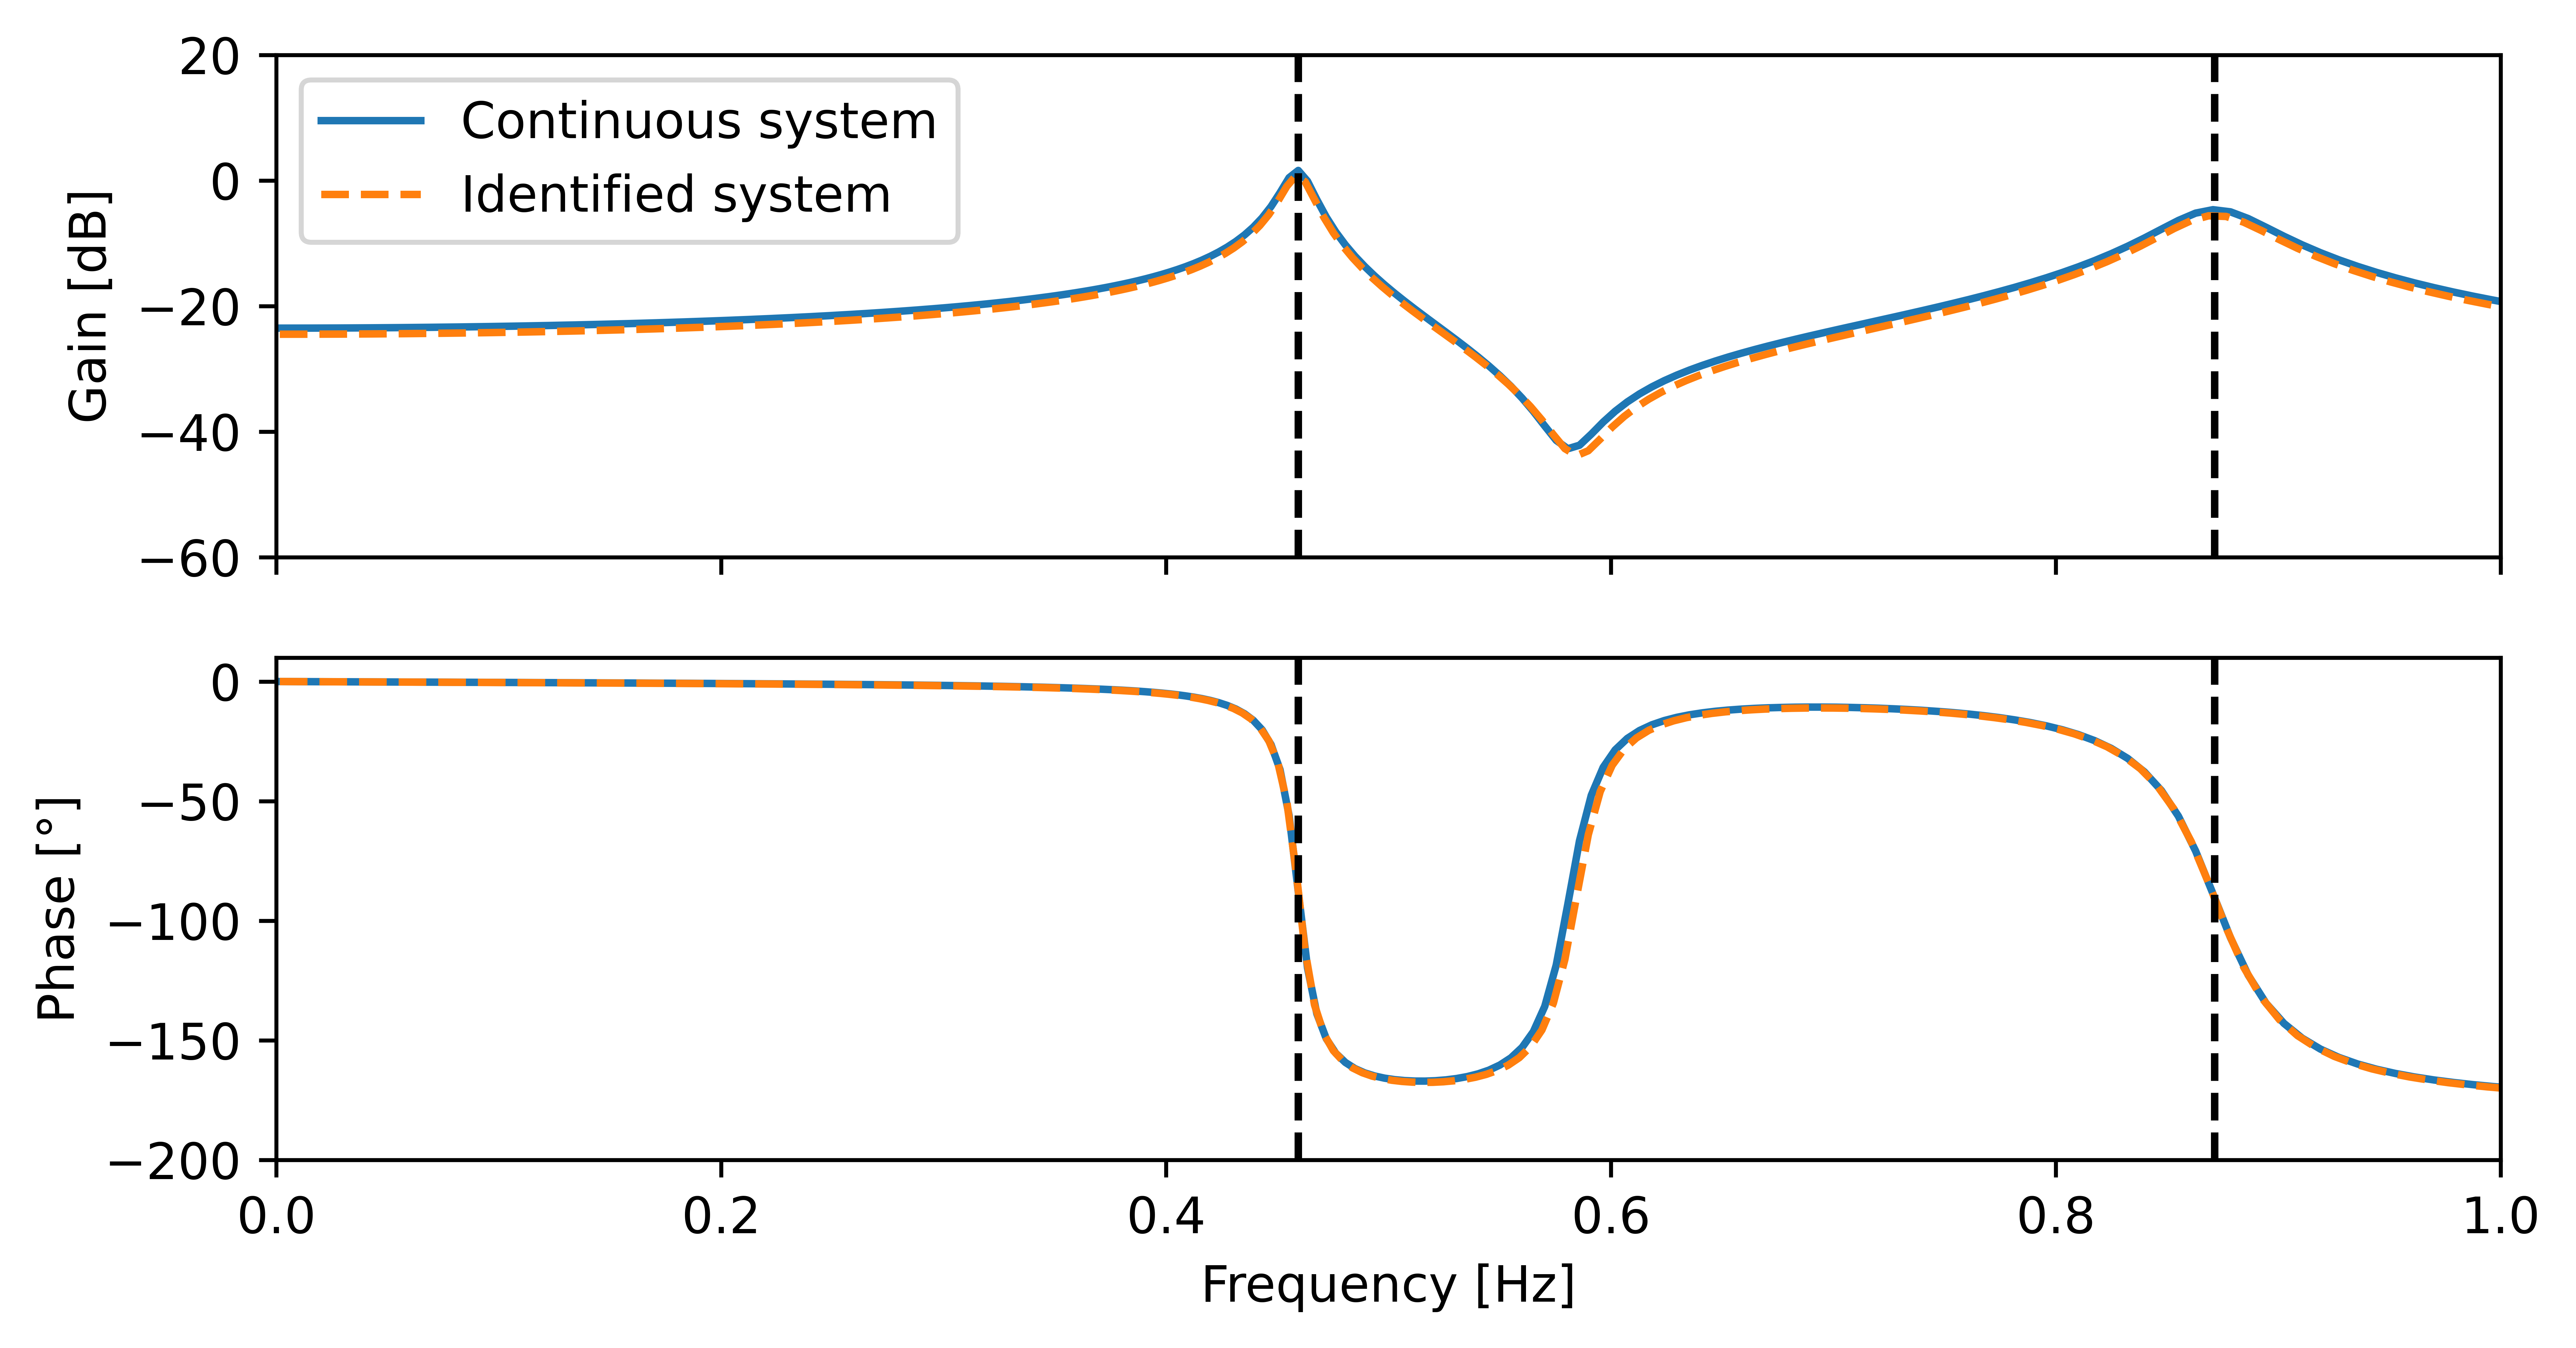
\includegraphics[width=.8\textwidth]{identified_rfr.png}
    \vfill
\end{frame}

\begin{frame}
    \frametitle{Model Predictive Control}
    \vfill
    \begin{minipage}{.48\textwidth}
        \[
        \begin{aligned}
            \minimize & \quad \dfrac12 \sum_{t=0}^{\tau} \norm{\vb{y}_t}^2_{\vb{Q}} + \norm{\vb{u}_t}^2_{\vb{R}} \\
            \subto & \quad \vb{x}_{t+1} = \vb{Ax}_t + \vb{Bu}_t \\
                   & \quad \vb{y}_t = \vb{Cx}_t + \vb{Du}_t \\
                   & \quad \vb{y}_t \in \mathcal{Y}_t \\
                   & \quad \vb{u}_t \in \mathcal{U}_t
        \end{aligned}
        \]
    \end{minipage}%
    \hfill
    \begin{minipage}{.48\textwidth}
        \begin{itemize}
            \item Golden standard in industry-grade control.
            \item Very flexible framework w/ excellent performances.
            \item If $\mathcal{Y}_t$ and $\mathcal{U}_t$ are \emph{convex sets}, the whole optimization problem is convex.
        \end{itemize}
    \end{minipage}
    \vfill
\end{frame}

\begin{frame}[standout, plain]
    \usebeamerfont{title}
    Linear System Identification

    \usebeamerfont{subtitle}
    A behavorial approach
\end{frame}

\begin{frame}[t, c]{Single Input/Single Output setup}
    \vfill
    \begin{minipage}{.48\textwidth}
        \centering
        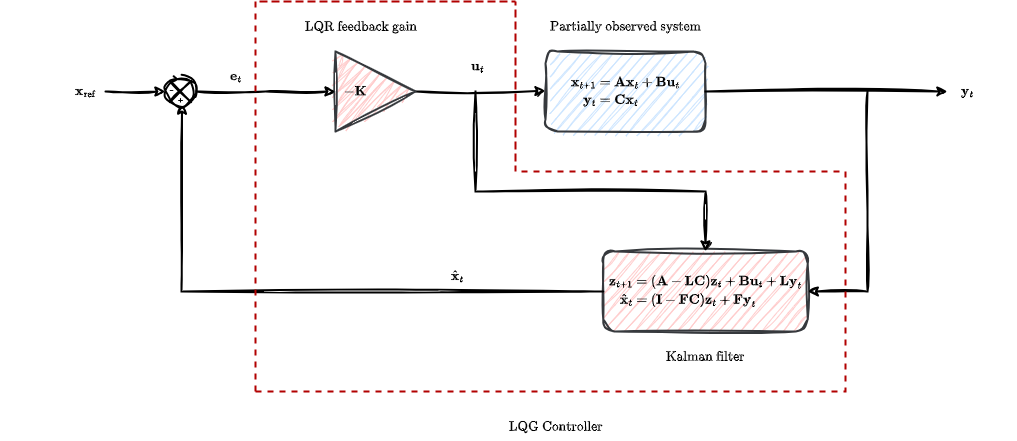
\includegraphics[width=\textwidth]{LQG_controller.png}
    \end{minipage}%
    \hfill
    \begin{minipage}{.48\textwidth}
        \centering
        \underline{\textbf{Hypothesis}}
        \par\bigskip
        \begin{itemize}
            \item   The true system $\Sigma$ is unknown.
            \item   Its input-output dynamics can be well approximated by an LTI model.
            \item   The rank of the model is unknown.
            \item   Only input-output data are available.
        \end{itemize}
    \end{minipage}
    \vfill
\end{frame}

\begin{frame}[t, c]{A behavorial view of LTI systems}
    \vfill
    \begin{minipage}{.68\textwidth}
        \begin{definition}
            A discrete-time \textbf{dynamical system} is defined by\\ a 3-tuple $\Sigma = (\mathbb{Z}_+, \mathbb{W}, \mathcal{B})$ where
            %
            \par\bigskip
            %
            \begin{enumerate}
                \item   $\mathbb{Z}_+$ is the discrete-time axis.
                \item   $\mathbb{W}$ is the signal space.
                \item   $\mathcal{B} \subseteq \mathbb{W}^{\mathbb{Z}_+}$ is the \emph{behavior}.
            \end{enumerate}
        \end{definition}
    \end{minipage}%
    \hfill
    \begin{minipage}{.28\textwidth}
        \centering
        
\includegraphics[width=\textwidth]{willems_book.jpg}
    \end{minipage}
    \vfill
\end{frame}

\begin{frame}[t, c]{A behavorial view of LTI systems}
    \vfill
    \begin{minipage}{.68\textwidth}
        \begin{definition}
            The dynamical system $\Sigma = \left( \mathbb{Z}_+, \mathbb{W}, \mathcal{B} \right)$ is
            %
            \par\bigskip
            %
            \begin{enumerate}
                \item   \textbf{linear} if $\mathbb{W}$ is a vector space and $\mathcal{B} \subseteq \mathbb{W}^{\mathbb{Z}_+}$ is a subspace.
                \item   \textbf{time-invariant} if $\sigma \mathcal{B} \subseteq \mathcal{B}$ where $\sigma w_t = w_{t+1}$.
                \item   \textbf{complete} if $\mathcal{B}$ is closed $\leftrightarrow$ $\mathbb{W}$ is finite dimensional.
            \end{enumerate}
        \end{definition}
    \end{minipage}%
    \hfill
    \begin{minipage}{.28\textwidth}
        \centering
        
\includegraphics[width=\textwidth]{willems_book.jpg}
    \end{minipage}
    \vfill
\end{frame}

\begin{frame}[t, c]{A behavorial view of LTI systems}
    \vfill
    Informally, the behavior $\mathcal{B}$ is the solution set of the linear difference equation describing the system, \ie
    %
    \[
        \mathcal{B} \equiv \left\{ w \in \mathbb{W}^{\mathbb{Z}_+} \quad \vert \quad R(\sigma) w = 0 \right\},
    \]
    %
    where $R \in \mathbb{R}^{g \times q}\left[\sigma\right]$ is a \emph{polynomial matrix} (if $\mathbb{W} = \mathbb{R}^q$).
    This is known as the \emph{kernal representation} of the system.
    \vfill
\end{frame}

\begin{frame}[t, c]{Input-Output LTI systems}
    \vfill
    If the polynomial matrix $R \in \R^{g \times q}\left[\sigma\right]$ is rank-deficient, the signal $w$ can be partitioned as $w = \mathrm{col}(u, y) \in \mathcal{B}^u \times \mathcal{B}^y$, where $u$ is the input and $y$ the output. Then
    %
    \[
        \begin{bmatrix} -Q(\sigma) & P(\sigma) \end{bmatrix} \colvec{u, y} = 0  \quad \leftrightarrow   \quad   a_0 y_t + \cdots + a_n y_{t+n} = b_0 u_t + \cdots b_n u_{t+n}.
    \]
    %
    The kernel representation of the I/O system is an \emph{AutoRegressive with Moving Average} (ARMA) model.
    \vfill
\end{frame}

\begin{frame}[t, c]{Input-Output LTI systems}
    \vfill
    \centering
    \[
        \mathcal{H}_{\tau} \left( \colvec{u, y} \right)
        =
        \begin{bmatrix}
            \colvec{u_1, y_1} & \colvec{u_2, y_2} & \colvec{u_3, y_3} & \cdots & \colvec{u_{T-\tau+1}, y_{T-\tau+1}} \\
            \colvec{u_2, y_2} & \colvec{u_3, y_3} & \colvec{u_4, y_4} & \cdots & \vdots \\
            \colvec{u_3, y_3} & \colvec{u_4, y_4} & \colvec{u_5, y_5} & \cdots & \vdots \\
            \vdots & \ddots & \ddots & \ddots & \vdots \\
            \colvec{u_{\tau}, y_{\tau}} & \cdots & \cdots & \cdots & \colvec{u_T, y_T}
        \end{bmatrix}
    \]
    %
    $\rowvec{b_0, a_0, \cdots, b_{\tau}, a_{\tau}}$ spans the left nullspace of this $\textbf{Hankel}$ matrix.
    \vfill
\end{frame}

\begin{frame}[t, c]{Fundamental Lemma}
    \vfill
    \begin{lemma}[Willems \etal, '05]
        Let $T, \tau \in \mathbb{Z}_{+}$. Consider
        \par\bigskip
        \begin{itemize}
            \item a \emph{controllable} LTI system $\Sigma = \left( \mathbb{Z}_{+}, \mathbb{R}^{p+q}, \mathcal{B} \right)$,
            \item a $T$-sample long trajectory $\mathrm{col}(u_d, y_d) \in \mathcal{B}_T$ where $u$ is \emph{persistently exciting} of order $\tau+n$ (prediction span + \# states).
        \end{itemize}
        \par\bigskip
        Then
        %
        \[
            \mathrm{colspan}\left( \mathcal{H}_{\tau} \left( \colvec{u, y} \right) \right) = \mathcal{B}_{\tau}.
        \]
    \end{lemma}
    \vfill
\end{frame}

\begin{frame}
    \vfill
    \begin{minipage}{.32\textwidth}
        \[
            \begin{aligned}
                \vb{x}_{t+1} & = \vb{Ax}_t + \vb{Bu}_t \\
                \vb{y}_t & = \vb{Cx}_t + \vb{Du}_t
            \end{aligned}
        \]
    \end{minipage}%
    \hfill
    \begin{minipage}{.18\textwidth}
    $$\Longleftrightarrow$$
    \end{minipage}%
    \begin{minipage}{.46\textwidth}
        \[
            \mathrm{colspan}\left(
            \begin{bmatrix}
                \colvec{u_1, y_1} & \colvec{u_2, y_2} & \colvec{u_3, y_3} & \cdots \\
                \colvec{u_2, y_2} & \colvec{u_3, y_3} & \colvec{u_4, y_4} & \cdots \\
                \colvec{u_3, y_3} & \colvec{u_4, y_4} & \colvec{u_5, y_5} & \cdots \\
                \vdots & \ddots & \ddots & \ddots
            \end{bmatrix}
            \right)
        \]
    \end{minipage}

    \begin{minipage}{.32\textwidth}
        \centering
        Parametric state-space model
    \end{minipage}%
    \hfill
    \begin{minipage}{.18\textwidth}
    \end{minipage}%
    \hfill
    \begin{minipage}{.46\textwidth}
        \centering
        Non-parametric model from raw data
    \end{minipage}
    \vfill
\end{frame}

\begin{frame}
    \frametitle{Data-driven simulation}
    \vfill
    \underline{\textbf{Problem --}} Predict future output ${\color{red}{y}} \in \mathbb{R}^{q \cdot \tau}$ based on
    %
    \begin{itemize}
        \item Training data $\mathrm{col}(u^d, y^d) \in \mathcal{B}_{T_{\mathrm{data}}}$ {\color{gray} $\to$ Form Hankel matrix.}
        \item Initial trajectory $\mathrm{col}(u_{\mathrm{ini}}, y_{\mathrm{ini}}) \in \mathbb{R}^{(p+q) \cdot T_{\mathrm{ini}}}$ {\color{gray} $\to$ Estimate initial condition $\vb{x}_{\mathrm{ini}}$.}
        \item Input signal ${\color{blue}{u}} \in \R^{p \cdot \tau}$ {\color{gray} $\to$ Predict forward.}
    \end{itemize}
    \vfill
\end{frame}

\begin{frame}
    \vfill
    \underline{\textbf{Solution --}} Given $\color{blue}\left( u_1, u_2, \cdots, u_{\tau} \right)$ and $\mathrm{col}(u_{\mathrm{ini}}, y_{\mathrm{ini}})$, compute $\vb{g}$ and $\color{red}\left( y_1, y_2, \cdots, y_{\tau} \right)$ from
    %
    \[
        \colvec{\vb{U}_p, \vb{Y}_p, {\color{blue} \vb{U}_f}, {\color{red} \vb{Y}_f}} \vb{g}
        = \colvec{u_{\mathrm{ini}}, y_{\mathrm{ini}}, {\color{blue} u}, {\color{red} y}}.
    \]
    %
    If $T_{\mathrm{ini}} \geq \text{lag}$ of the system then $\color{red} y$ is unique.
    \vfill
\end{frame}

\begin{frame}
    \vfill
    \underline{\textbf{Step 1}} -- The vector $\vb{g}$ is given by
    %
    \[
        \vb{g} = \colvec{\vb{U}_p, \vb{Y}_p, \vb{U}_f}^{\dagger} \colvec{u_{\mathrm{ini}}, y_{\mathrm{ini}}, u}.
    \]
    %
    \vfill
    \underline{\textbf{Step 2}} - The future output $\color{red} y$ is then given by
    %
    \[
        {\color{red} y} = \vb{Y}_f \vb{g}.
    \]
    \vfill
\end{frame}

\begin{frame}
    \vfill
    \centering
    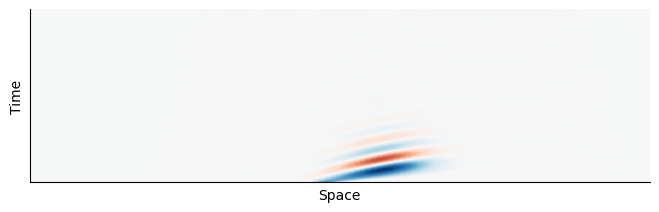
\includegraphics[width=.8\textwidth]{space_time_diagram_input.png}
    \par
    \[
        \dfrac{\partial u}{\partial t} = \left( -\nu \dfrac{\partial}{\partial x} + \gamma \dfrac{\partial^2}{\partial x^2} + \mu(x) \right) u + f
    \]
    \vfill
\end{frame}

\begin{frame}
    \centering
    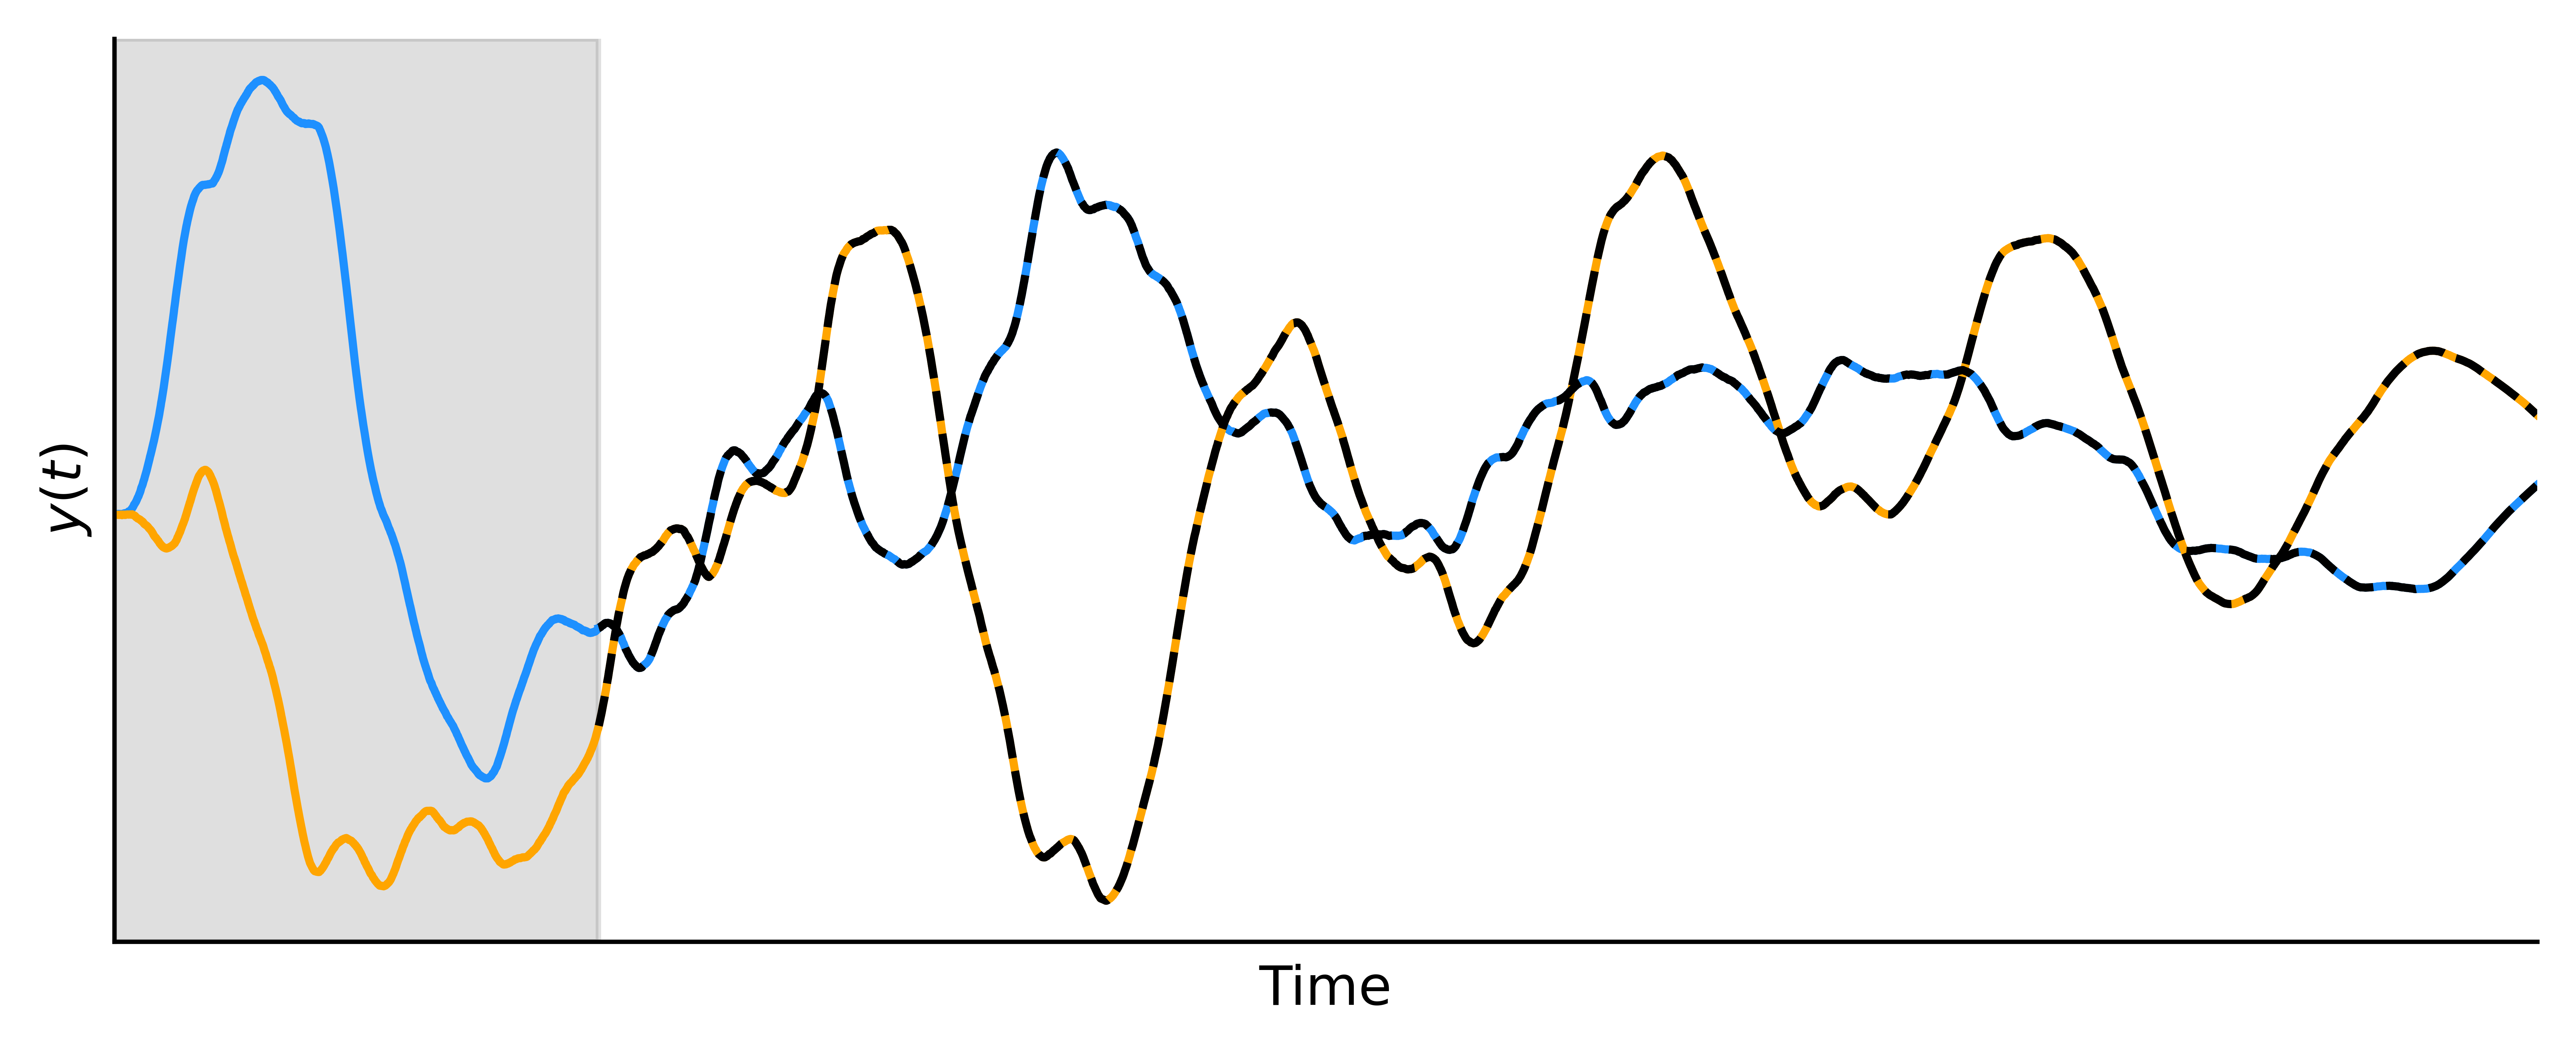
\includegraphics[width=.9\textwidth]{data_driven_simulation.png}
\end{frame}

\begin{frame}
    \frametitle{Data-Enabled Predictive Control (DeePC)}
    \vfill
    \begin{minipage}{.48\textwidth}
        \[
        \begin{aligned}
            \minimize_{\vb{g}, \vb{y}, \vb{u}} & \quad \dfrac12 \sum_{t=0}^{\tau} \norm{\vb{y}_t}^2_{\vb{Q}} + \norm{\vb{u}_t}^2_{\vb{R}} \\
            \subto & \quad \colvec{\vb{U}_p, \vb{Y}_p, \vb{U}_p, \vb{U}_f} \vb{g} = \colvec{\vb{u}_{\mathrm{ini}}, \vb{y}_{\mathrm{ini}}, \vb{u}, \vb{y}}, \\
                   & \quad \vb{y}_t \in \mathcal{Y}_t, \\
                   & \quad \vb{u}_t \in \mathcal{U}_t.
        \end{aligned}
        \]
    \end{minipage}%
    \hfill
    \begin{minipage}{.48\textwidth}
        \begin{itemize}
            \item Non-parametric model for \emph{prediction} and \emph{estimation}.
            \item Very flexible framework w/ excellent performances.
            \item If $\mathcal{Y}_t$ and $\mathcal{U}_t$ are \emph{convex sets}, the whole optimization problem is convex.
            \item Equivalent to MPC if $\Sigma$ is a deterministic LTI system.
        \end{itemize}
    \end{minipage}
    \vfill
\end{frame}

\begin{frame}
    \vfill
    \begin{minipage}{.68\textwidth}
        \begin{itemize}
            \item   Parameterization of the IO behavior is irrelevant as long as it captures $\mathcal{B} = \mathcal{B}^u \times \mathcal{B}^y$ correctly.
                %
            \item   Even when the maths are well understood, some things fundamentally stay out of reach, no matter how fancy of a data-driven algorithm you use.
                %
            \item   A proper choice of sensors and actuators is thus crucial to maximize the amount of information one can extract from data.
        \end{itemize}
    \end{minipage}%
    \hfill
    \begin{minipage}{.28\textwidth}
        \centering
        
\includegraphics[width=\textwidth]{conclusion.png}
    \end{minipage}
    \vfill
\end{frame}

\section{Nonlinear System Identification}

\begin{frame}[standout, plain]
    \usebeamerfont{title}
    Sparse Identification of Nonlinear Dynamics

    \usebeamerfont{subtitle}
    A practical approach
\end{frame}

\begin{frame}
    \frametitle{What is SINDy?}
    \begin{minipage}{.28\textwidth}
        \centering
        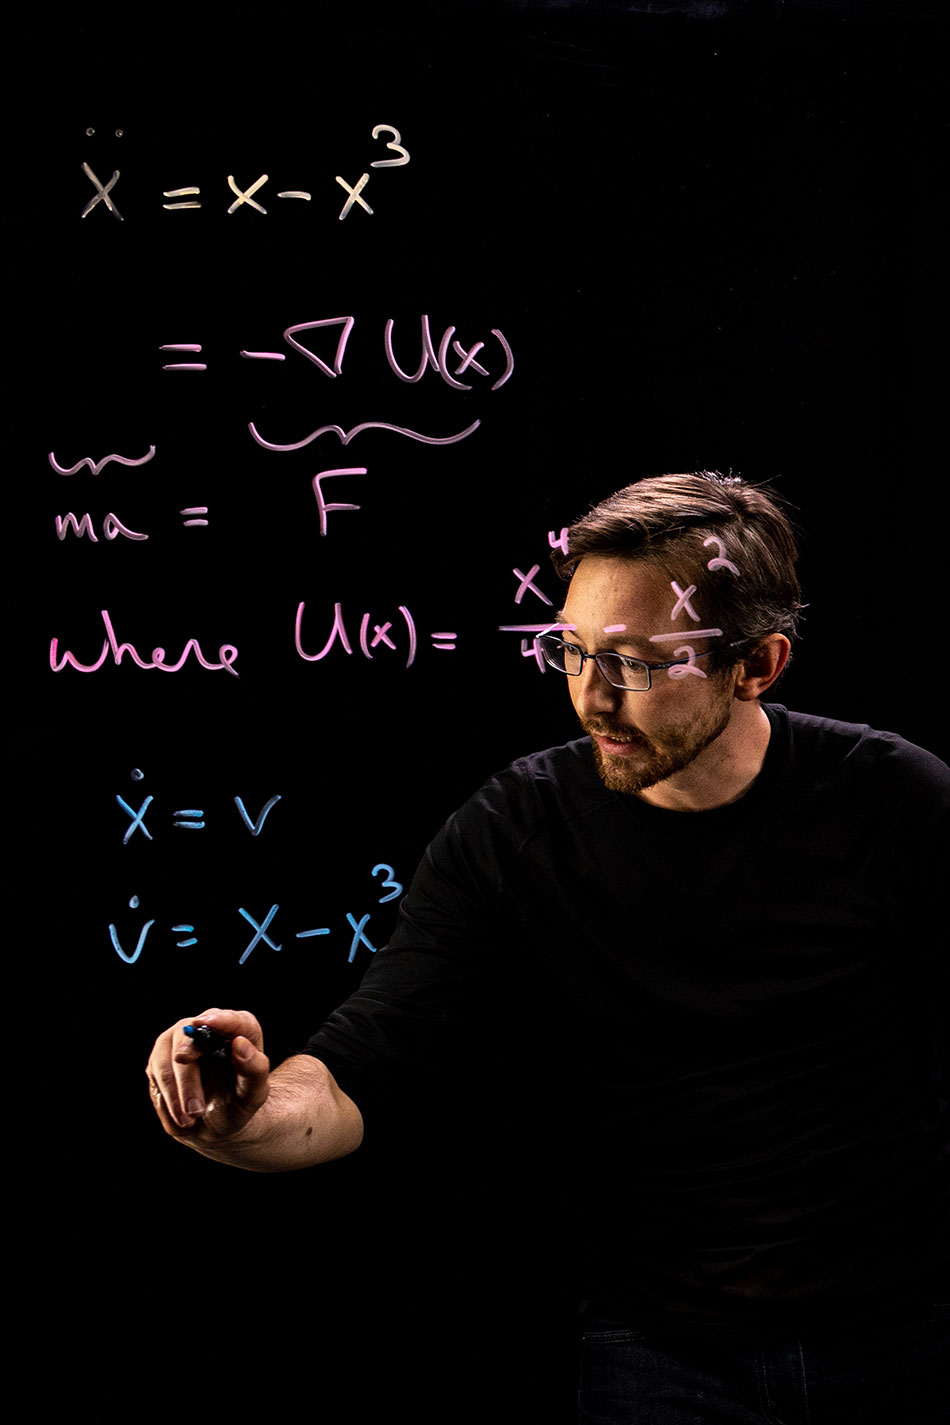
\includegraphics[width=\textwidth]{imgs/steve.jpg}
        \tiny
        Steven Brunton (UW, USA)
    \end{minipage}%
    \hfill
    \begin{minipage}{.68\textwidth}
        \vspace{-2em}
        \begin{itemize}
            \item Stands for \emph{Sparse Identification of Nonlinear Dynamics}.
            \item First paper published in 2015 in PNAS.
            \item Framework for identifying equations from data leveraging \emph{sparse regression} algorithms.
            \item Developed into a complete ecosystem since the seminal work of Steve.
        \end{itemize}
    \end{minipage}
    \vfill
\end{frame}

\begin{frame}[plain]
    \vfill
    \begin{minipage}{.68\textwidth}
        \textbf{Observation} -- Using suitable coordinates, many systems in the physical sciences are described by a set of \textbf{sparse} equations.
    \end{minipage}%
    \hfill
    \begin{minipage}{.28\textwidth}
        \centering
        \begin{overprint}
            \onslide<1>
            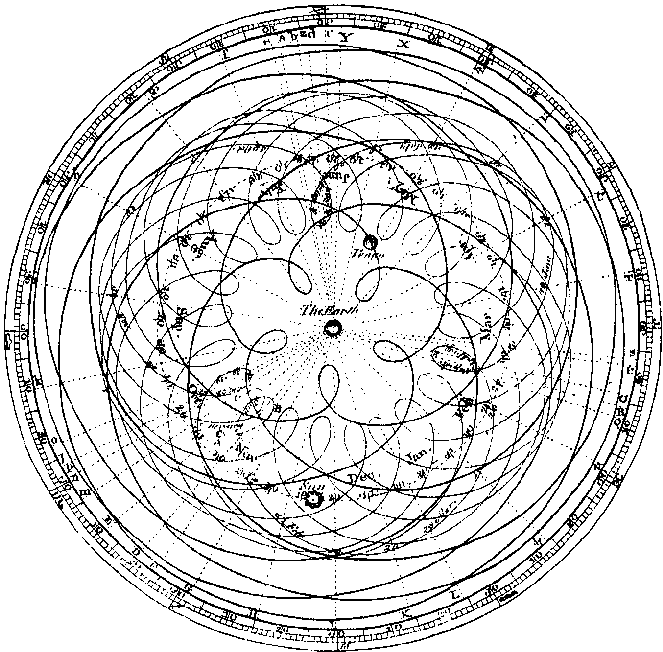
\includegraphics[width=\textwidth]{imgs/ptolemaic_system.png}
            \onslide<2>
            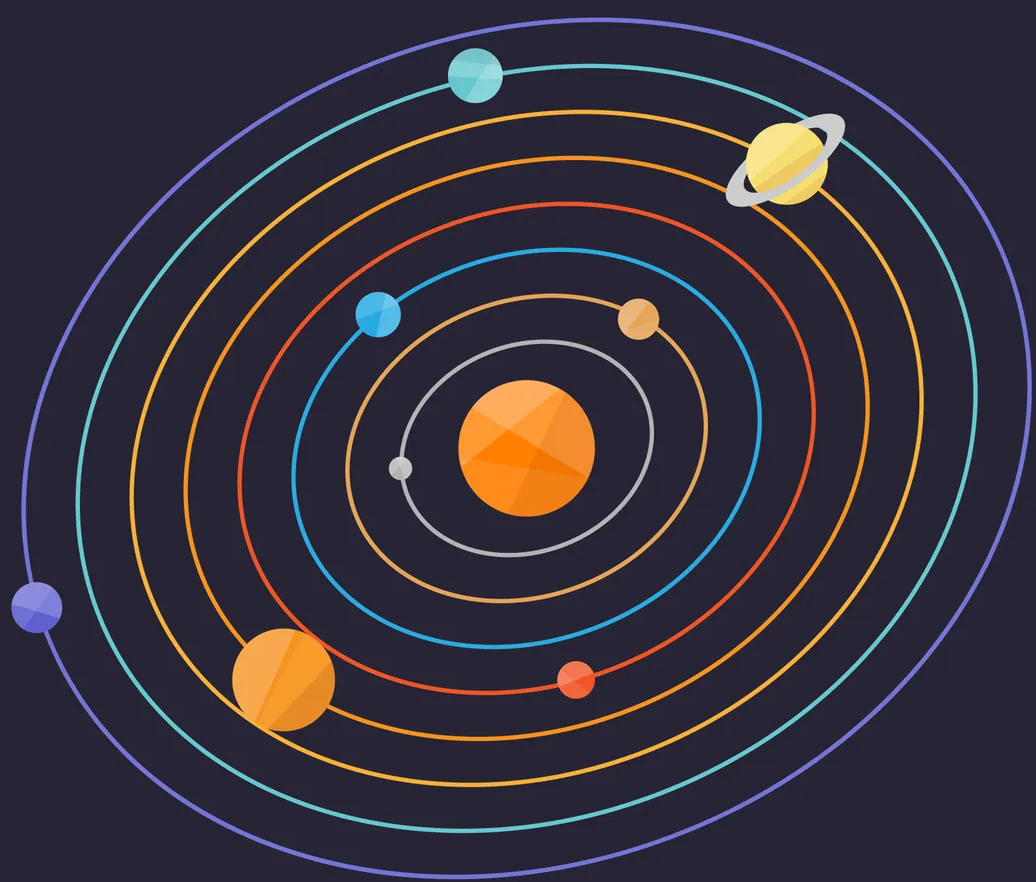
\includegraphics[width=\textwidth]{imgs/solar_system.png}
        \end{overprint}
    \end{minipage}
    \vfill
\end{frame}

\begin{frame}[plain]
    \vfill
    \centering
    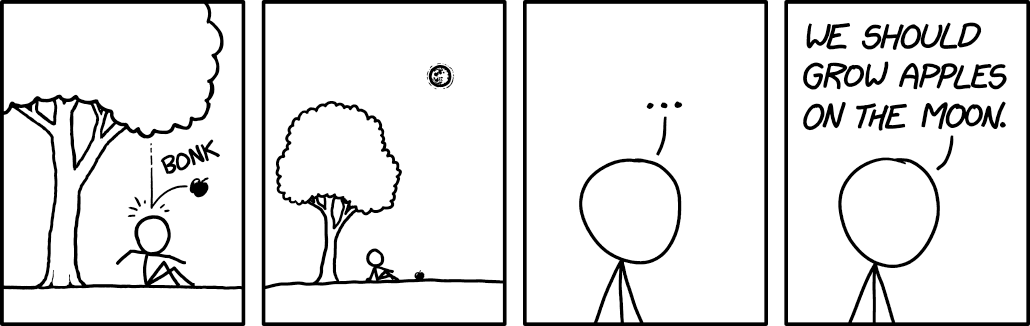
\includegraphics[width=.8\textwidth]{imgs/newton.png}
    \vfill
\end{frame}

\begin{frame}[standout, plain]
	\vfill
        \small
        \begin{multicols}{2}
            \begin{itemize}
                \item Vanilla SINDy
                \item Constrained SINDy
                \item Weak SINDy
                \item Ensemble SINDy
                \item SINDy for control
                \item SINDy-MPC
                \item SINDy-PI
                \item MANDy
                \item Langevin Regression
                \item Bayesian SINDy
                \item CINDy
                \item \ldots
            \end{itemize}
            \end{multicols}
    	\vfill
\end{frame}

\begin{frame}[standout, plain]
    \vfill
    \centering
    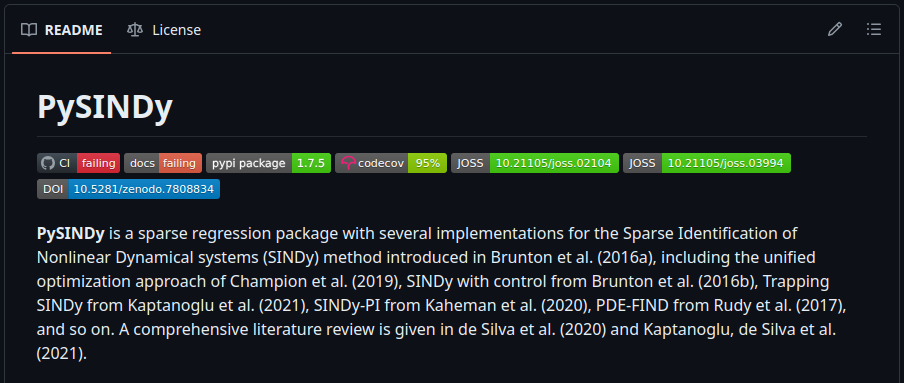
\includegraphics[width=.8\textwidth]{imgs/pysindy.png}
    \vfill
\end{frame}

\Section{SINDy for ODE}
\begin{frame}
    \frametitle{SINDy for Ordinary Diff. Eq.}
    \vfill
    \centering
    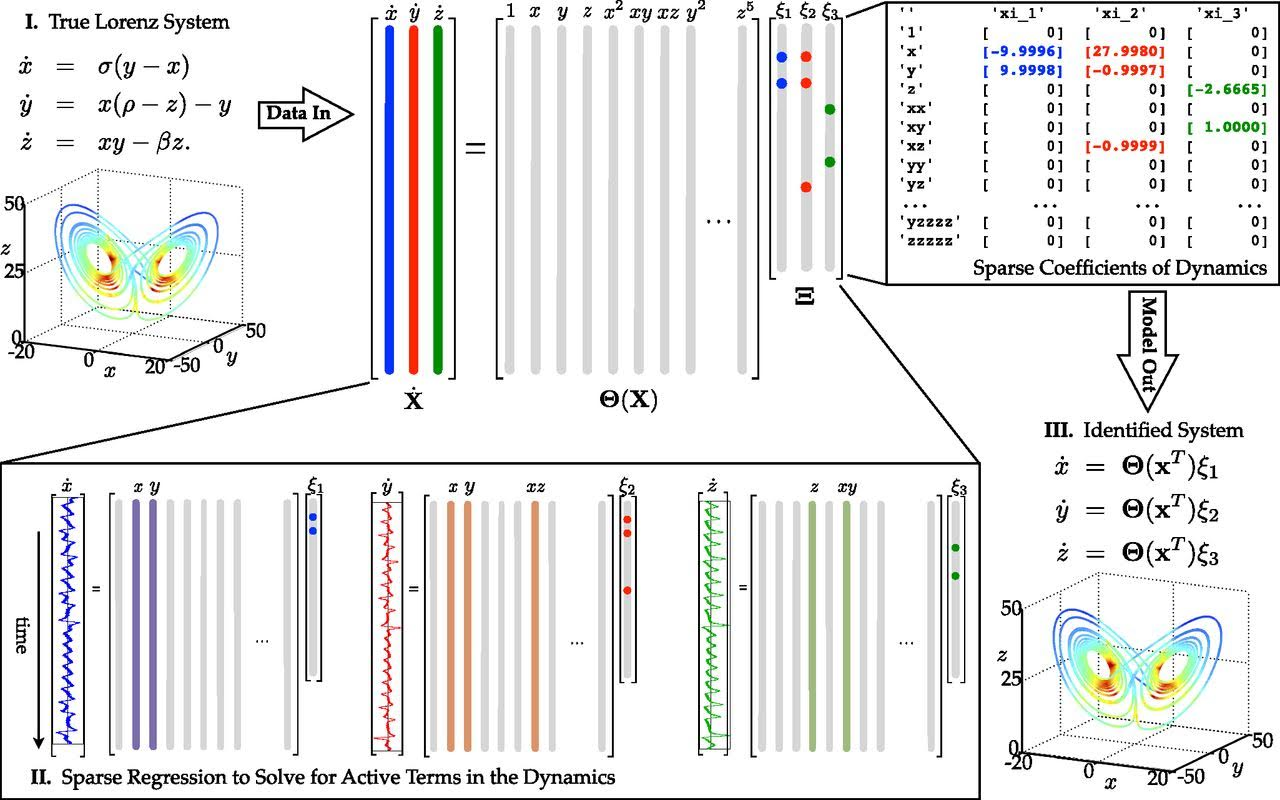
\includegraphics[height=.8\textheight]{imgs/sindy_paper.png}
    \vfill
\end{frame}

\begin{frame}
    \vfill
    \[
    \begin{aligned}
        \minimize_{\boldsymbol{\alpha}} & \quad \norm{\boldsymbol{\alpha}}_0                                                                 \\
        \subto                          & \int_{0}^T \left( \dot{\vb{x}} - f(\vb{x}) \right) \dd t = \allzeros \\
                                        & f(\vb{x}) - \sum_{i=1}^n \vartheta_i(\vb{x}) \alpha_i = \allzeros, \\
                                        & h(\vb{x}, \boldsymbol{\alpha}) = \allzeros \\
                                        & g(\vb{x}, \boldsymbol{\alpha}) \preccurlyeq \allzeros.
    \end{aligned}
    \]
    \vfill
\end{frame}

\begin{frame}
    \vfill
    \[
    \begin{aligned}
        \minimize_{\boldsymbol{\alpha}} & \quad \norm{\boldsymbol{\alpha}}_1 \\
        \subto                          & \norm{\dot{\vb{X}} - \boldsymbol{\Theta}(\vb{X}) \boldsymbol{\alpha}}_F^2 \leq \varepsilon \\
                                        & h(\vb{x}, \boldsymbol{\alpha}) = \allzeros                                                         \\
                                        & g(\vb{x}, \boldsymbol{\alpha}) \preccurlyeq \allzeros.
    \end{aligned}
    \]
    \vfill
\end{frame}

% \begin{frame}
%     \frametitle{Sparse calibration of a POD-Galerkin ROM}
%     \vfill
%     \begin{minipage}{.28\textwidth}
%         \centering
%         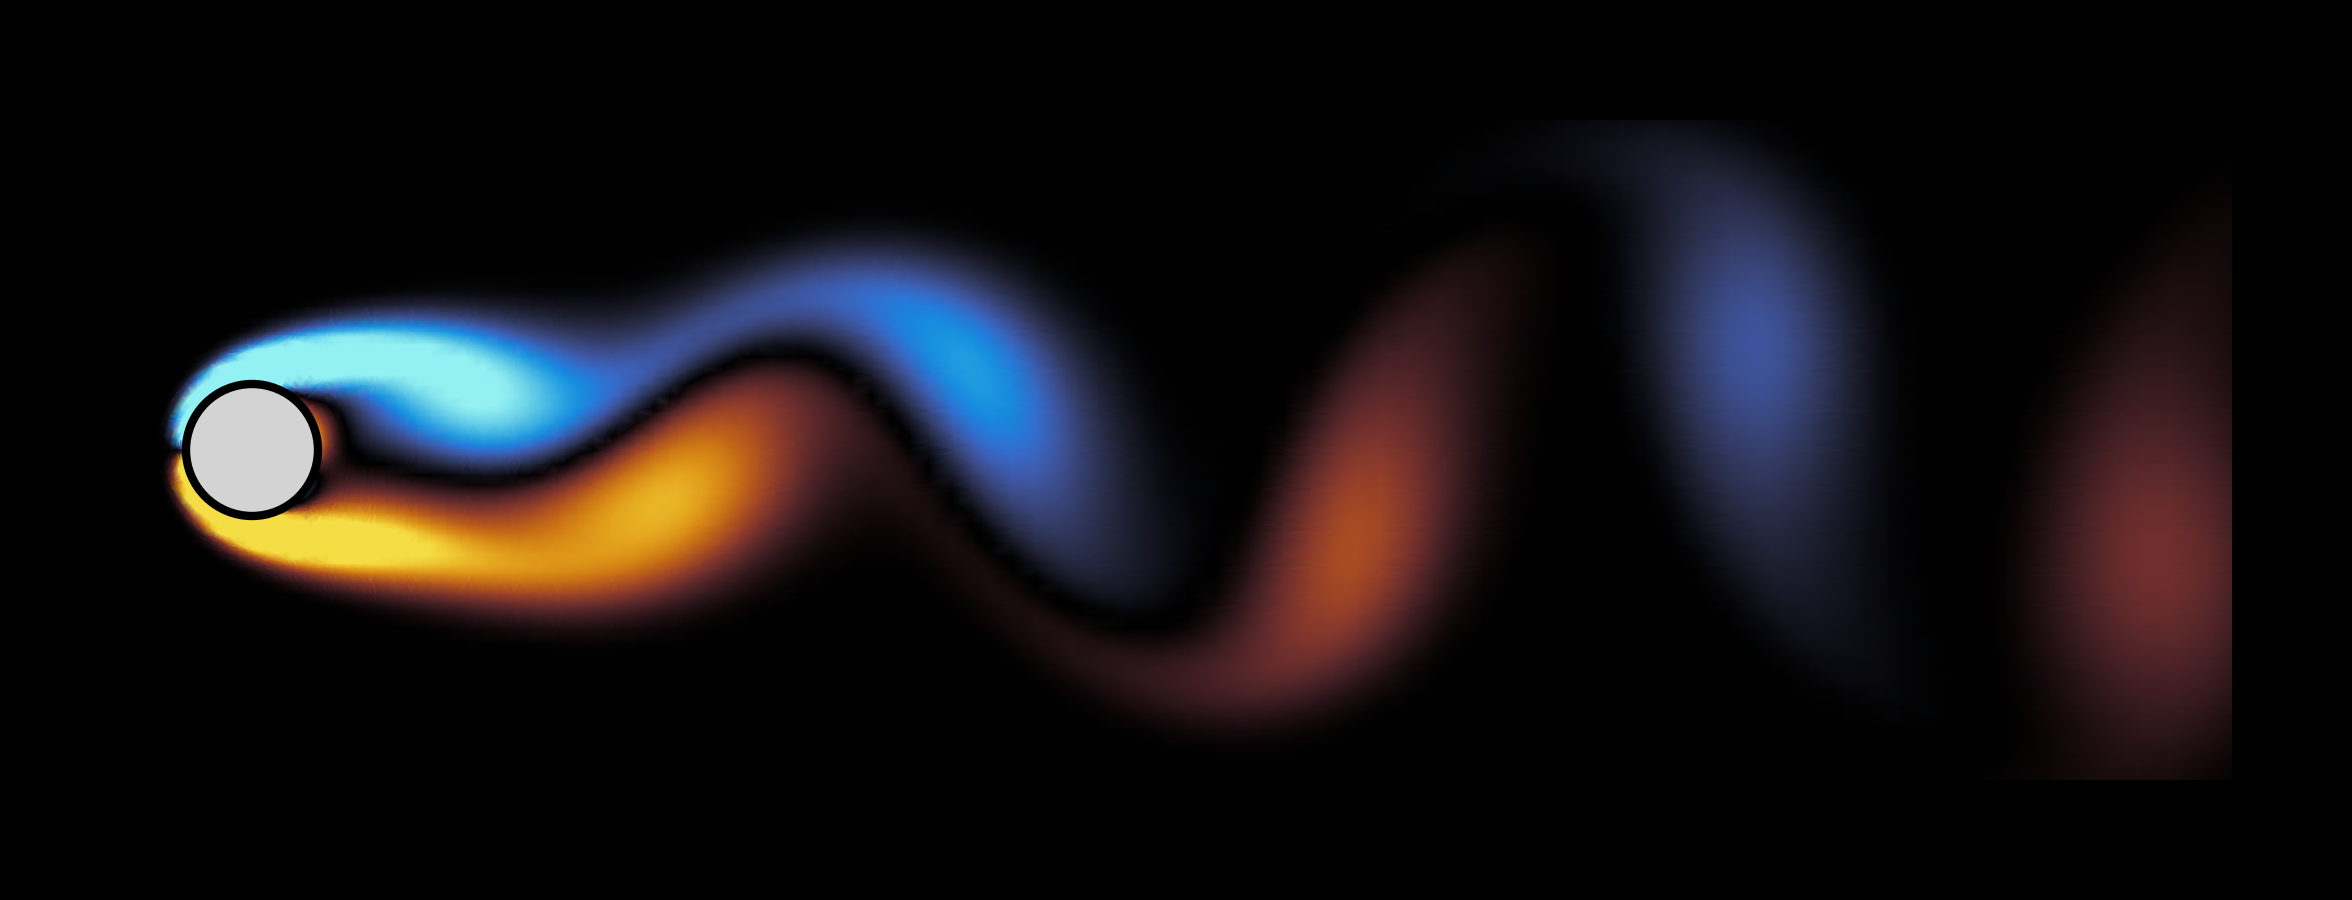
\includegraphics[height=.3\textheight, angle=-90, origin=c]{von_karman}
%     \end{minipage}%
%     \hfill
%     \begin{minipage}{.68\textwidth}
%         \centering
%         \textbf{POD-Galerkin ROM}
%         \[
%             \dot{x}_i = \sum_{j=1}^r L_{ij} x_j + \sum_{j, k=1}^r Q_{ijk} x_j x_k
%         \]
%     \end{minipage}
%     \vfill
% \end{frame}

% \begin{frame}
%     \vfill
%     \begin{minipage}{.48\textwidth}
%         \centering
%         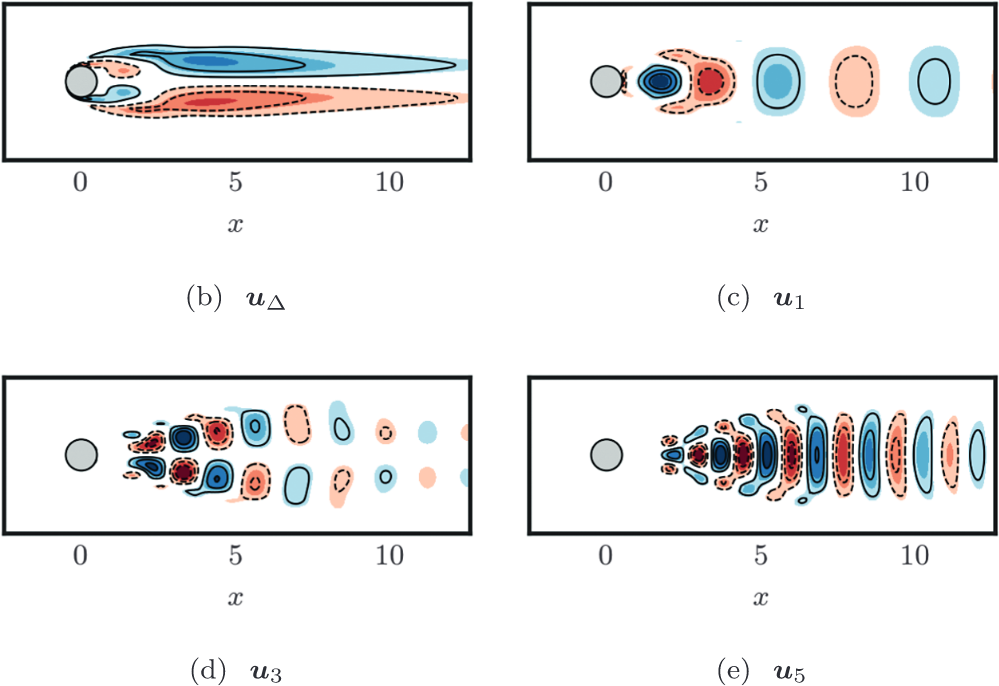
\includegraphics[width=\textwidth]{imgs/pod_cylinder.png}
%     \end{minipage}%
%     \hfill
%     \begin{minipage}{.48\textwidth}
%         \begin{itemize}
%             \item 3 POD modes capture 99\% of the variance.
%             \begin{itemize}
%                 \item Two for the von Kàrmàn vortex shedding.
%                 \item One for the distortion between the fixed point and the mean flow.
%             \end{itemize}
%             \par\bigskip
%             \item Yet, POD-Galerkin projection ROM has very limited accuracy.
%         \end{itemize}
%     \end{minipage}
%     \vfill
% \end{frame}

% \begin{frame}
%     \vfill
%     \centering
%     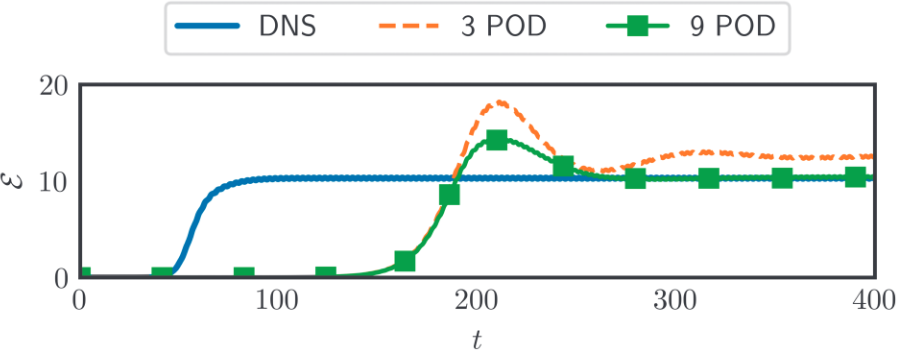
\includegraphics[width=\textwidth]{imgs/pod_galerkin_tke_cylinder.png}
%     \vfill
% \end{frame}

% \begin{frame}
%     \vfill
%     \centering
%     \textbf{"Normal form" POD-Galerkin ROM}
%     \bigskip
%     \[
%     \dot{x}_i = \sum_{j} L_{ij} x_j + \sum_{j, k} Q_{ijk} x_j x_k + \sum_{j, k, l} C_{ijkl} x_j x_k x_l
%     \]
%     \vfill
% \end{frame}

% \begin{frame}
%     \vfill
%     \begin{minipage}{.68\textwidth}
%         \begin{itemize}
%             \item Based from first principles and symmetry considerations:
%             %
%             \begin{itemize}
%                 \item $L_{ij} = \vb{u}_i^T \vb{A} \vb{u}_j$ is block-diagonal,
%                 \item $L_{33}$ is negative,
%                 \item $Q_{ijk}$ is skew-symmetric,
%                 \item $C_{ijkl}$ is dissipative.
%             \end{itemize}
%             \item All these lead to linear equality or inequality constraints.
%         \end{itemize}
%     \end{minipage}%
%     \hfill
%     \begin{minipage}{.28\textwidth}
    
%     \end{minipage}
%     \vfill
% \end{frame}

% \begin{frame}
%     \vfill
%     \[
%     \begin{aligned}
%         \minimize_{\bf{L}, \vb{Q}, \bf{C}} & \quad \norm{\bf{L}}_0 + \norm{\vb{Q}}_0 + \norm{\vb{C}}_0 \\
%         \subto                          & \norm{\dot{x}_i - L_{ij}x_j - Q_{ijk} x_j x_k - C_{ijkl} x_j x_k x_l }^2 \leq \varepsilon \\
%                                         & L_{1, 2} =  L_{1, 3} = 0, \\
%                                         & L_{2, 2} =  L_{2, 3} = 0, \\
%                                         & L_{3, 1} = L_{3, 2} = 0, \\
%                                         & L_{3, 3} \leq 0, \\
%                                         & Q_{iii} = Q_{ijk} - Q_{ikj} = 0, \\
%                                         & g(\vb{C}) \preccurlyeq \allzeros.
%     \end{aligned}
%     \]
%     \vfill
% \end{frame}

% \begin{frame}
%     \vfill
%     \centering
%     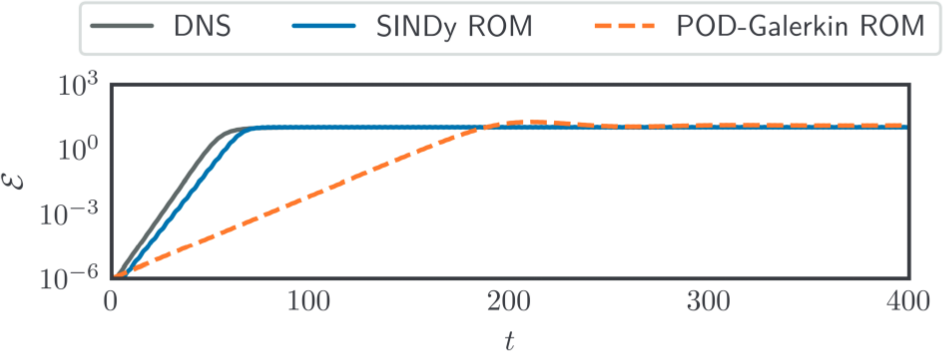
\includegraphics[width=\textwidth]{imgs/sindy_galerkin_tke_cylinder.png}
%     \vfill
% \end{frame}

% \begin{frame}
%     \vfill
%     \centering
%     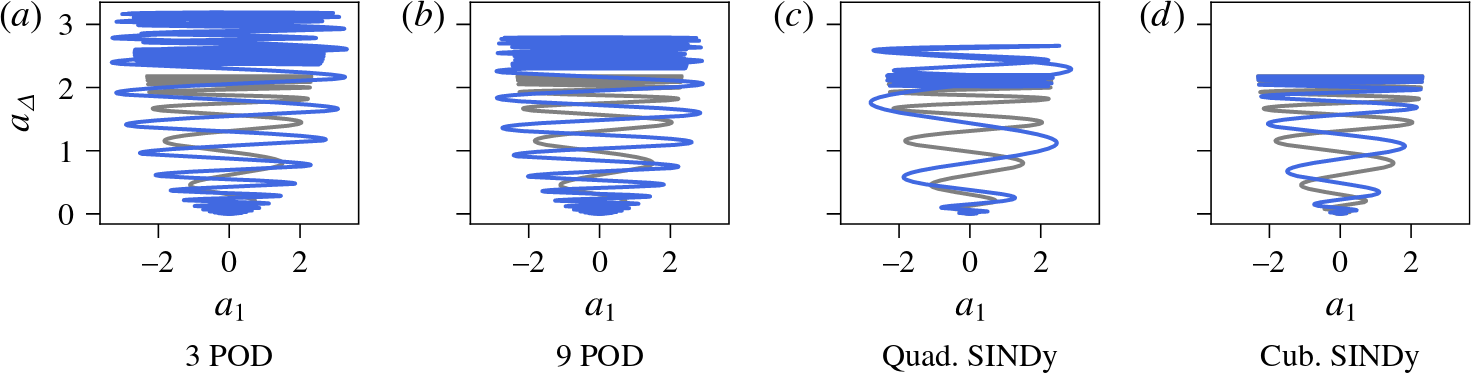
\includegraphics[width=\textwidth]{imgs/cylinder_attractor.png}
%     \vfill
% \end{frame}

\begin{frame}
    \frametitle{Identifying normal forms}
    \vfill
    \begin{minipage}{.38\textwidth}
        \centering
        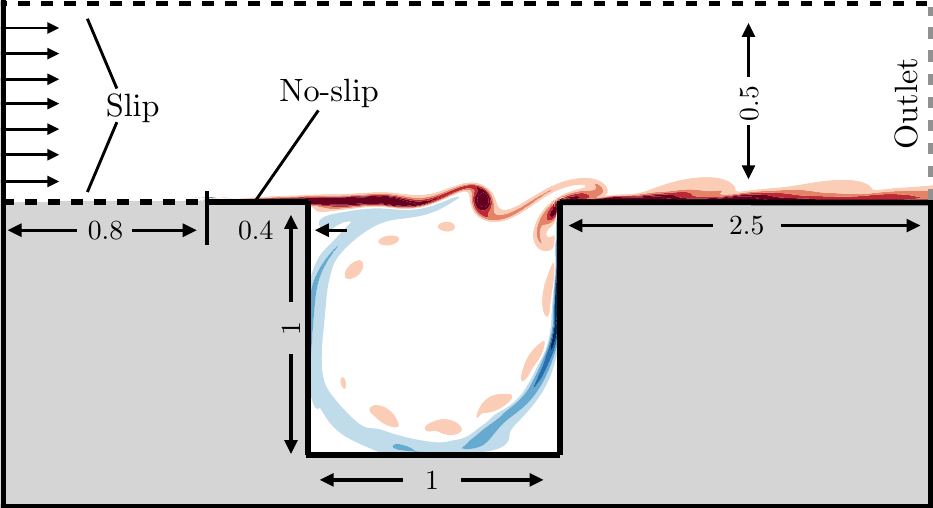
\includegraphics[width=\textwidth]{imgs/cavity_geomtry.png}
    \end{minipage}%
    \hfill
    \begin{minipage}{.58\textwidth}
        \begin{itemize}
            \item Classical example in flow control.
            \par\bigskip
            \item At $Re = 7500$, the dynamics are \emph{quasiperiodic}.
            \par\bigskip
            \item 64 POD modes required to capture 99\% of the fluctuations.
        \end{itemize}
    \end{minipage}
    \vfill
\end{frame}

\begin{frame}
    \vfill
    \centering
    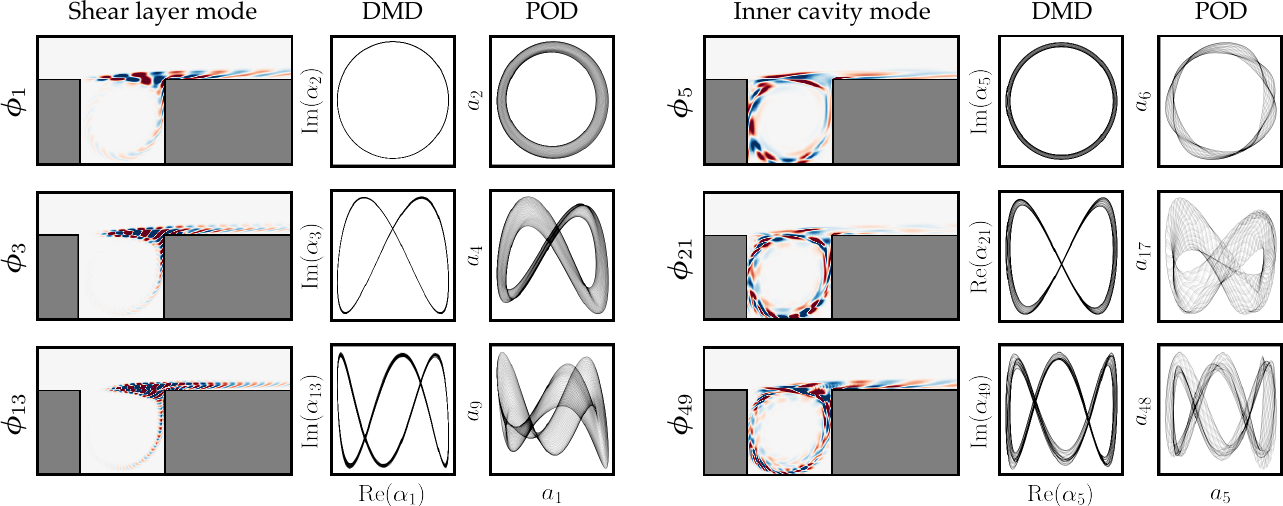
\includegraphics[width=\textwidth]{imgs/pod_modes.png}
    \vfill
\end{frame}

\begin{frame}
    \vfill
    \centering
    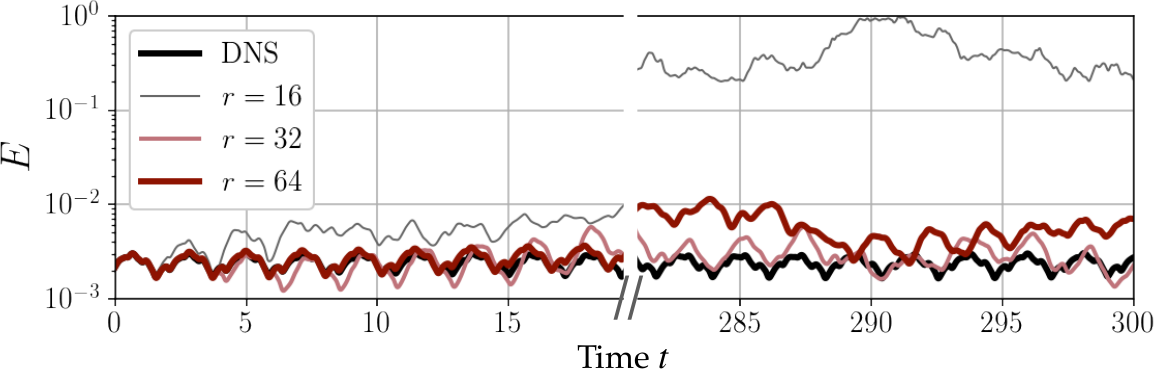
\includegraphics[width=\textwidth]{imgs/tke_galerkin.png}
    \vfill
\end{frame}

\begin{frame}
    \vfill
    \begin{minipage}{.48\textwidth}
        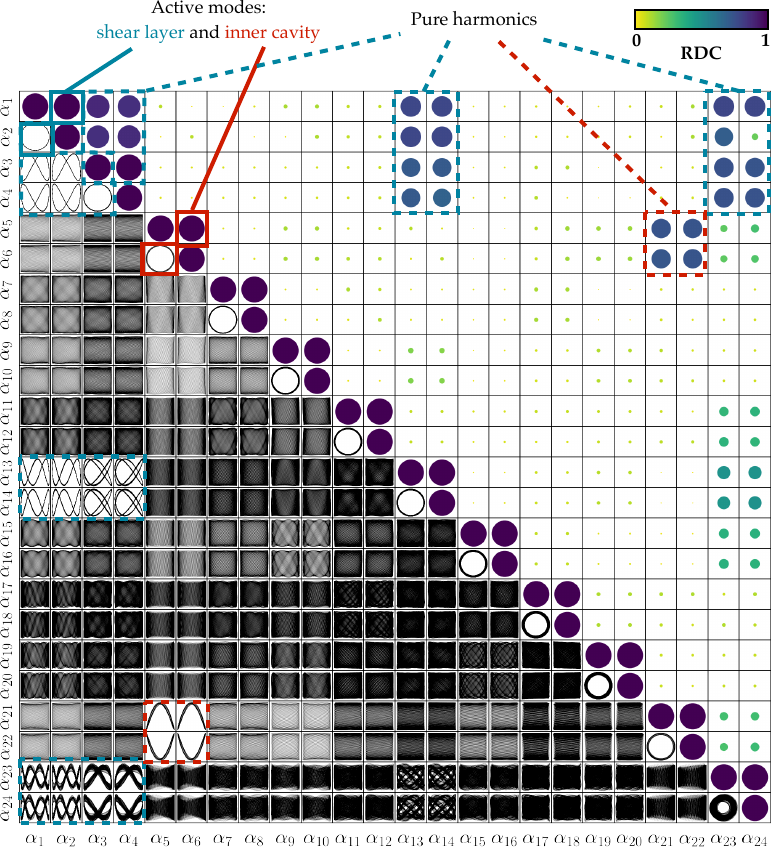
\includegraphics[width=\textwidth]{imgs/rdc_score.png}
    \end{minipage}%
    \hfill
    \begin{minipage}{.48\textwidth}
        \begin{itemize}
            \item Many modes are artifacts coming from representing a low-dimensional manifold in a large Euclidean space.
            \par\bigskip
            \item Need to find a way to break the \emph{Kolmogorov n-width}.
        \end{itemize}
    \end{minipage}
    \vfill
\end{frame}

\begin{frame}
    \vfill
    \begin{minipage}{.48\textwidth}
        \begin{itemize}
            \item Using only the four active degrees of freedom, SINDy identifies
            %
            \[
            \begin{aligned}
                \dot{x} & = \lambda_1 x - \mu_1 \abs{x}^2 x \\
                \dot{y} & = \lambda_2 y - \mu_2 \abs{y}^2 y.
            \end{aligned}
            \]
            \item ROM consistent with the known bifurcation diagram of the problem.
        \end{itemize}
    \end{minipage}%
    \hfill
    \begin{minipage}{.48\textwidth}
        \centering
        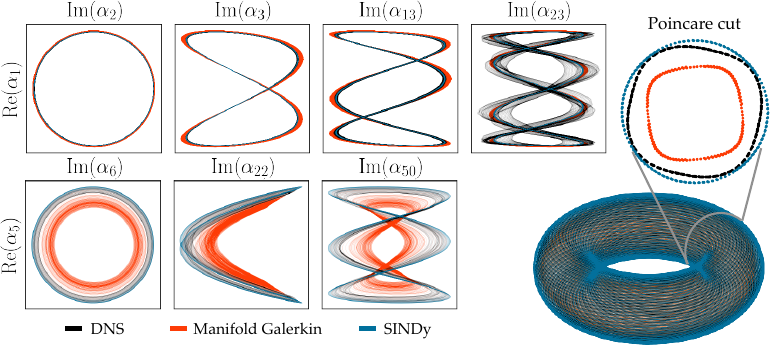
\includegraphics[width=\textwidth]{imgs/sindy_attractor.png}
    \end{minipage}
    \vfill
\end{frame}

\begin{frame}
    \vfill
    \centering
    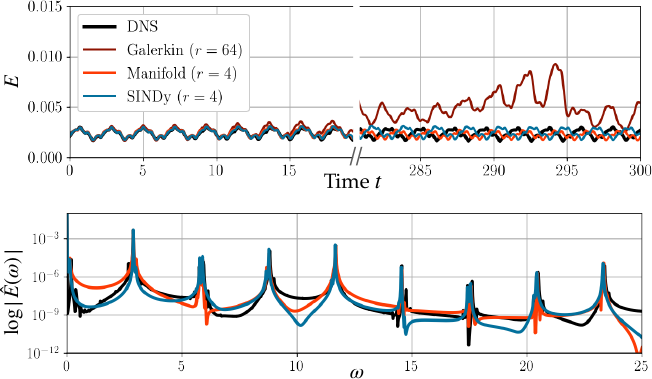
\includegraphics[width=.8\textwidth]{imgs/sindy_tke.png}
    \vfill
\end{frame}

\Section{Finding PDEs}
\begin{frame}
    \frametitle{SINDy for Partial Diff. Eq.}
    \vfill
    \begin{minipage}{.28\textwidth}
        \centering
        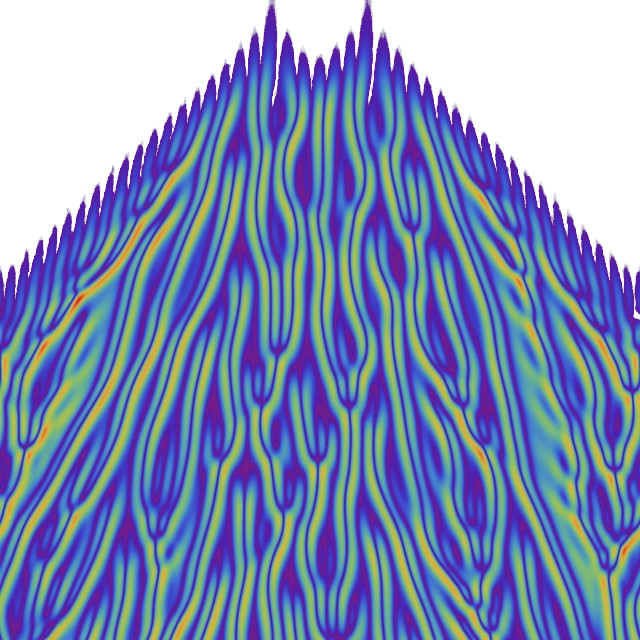
\includegraphics[width=\textwidth]{imgs/kuramoto.png}
    \end{minipage}%
    \hfill
    \begin{minipage}{.68\textwidth}
        \begin{itemize}
            \item Extending SINDy to PDE is straightforward.
            \par\bigskip
            \item Massively over-determined constrained least-squares problem.
        \end{itemize}
    \end{minipage}
    \vfill
\end{frame}

\begin{frame}
    \vfill
    \centering
    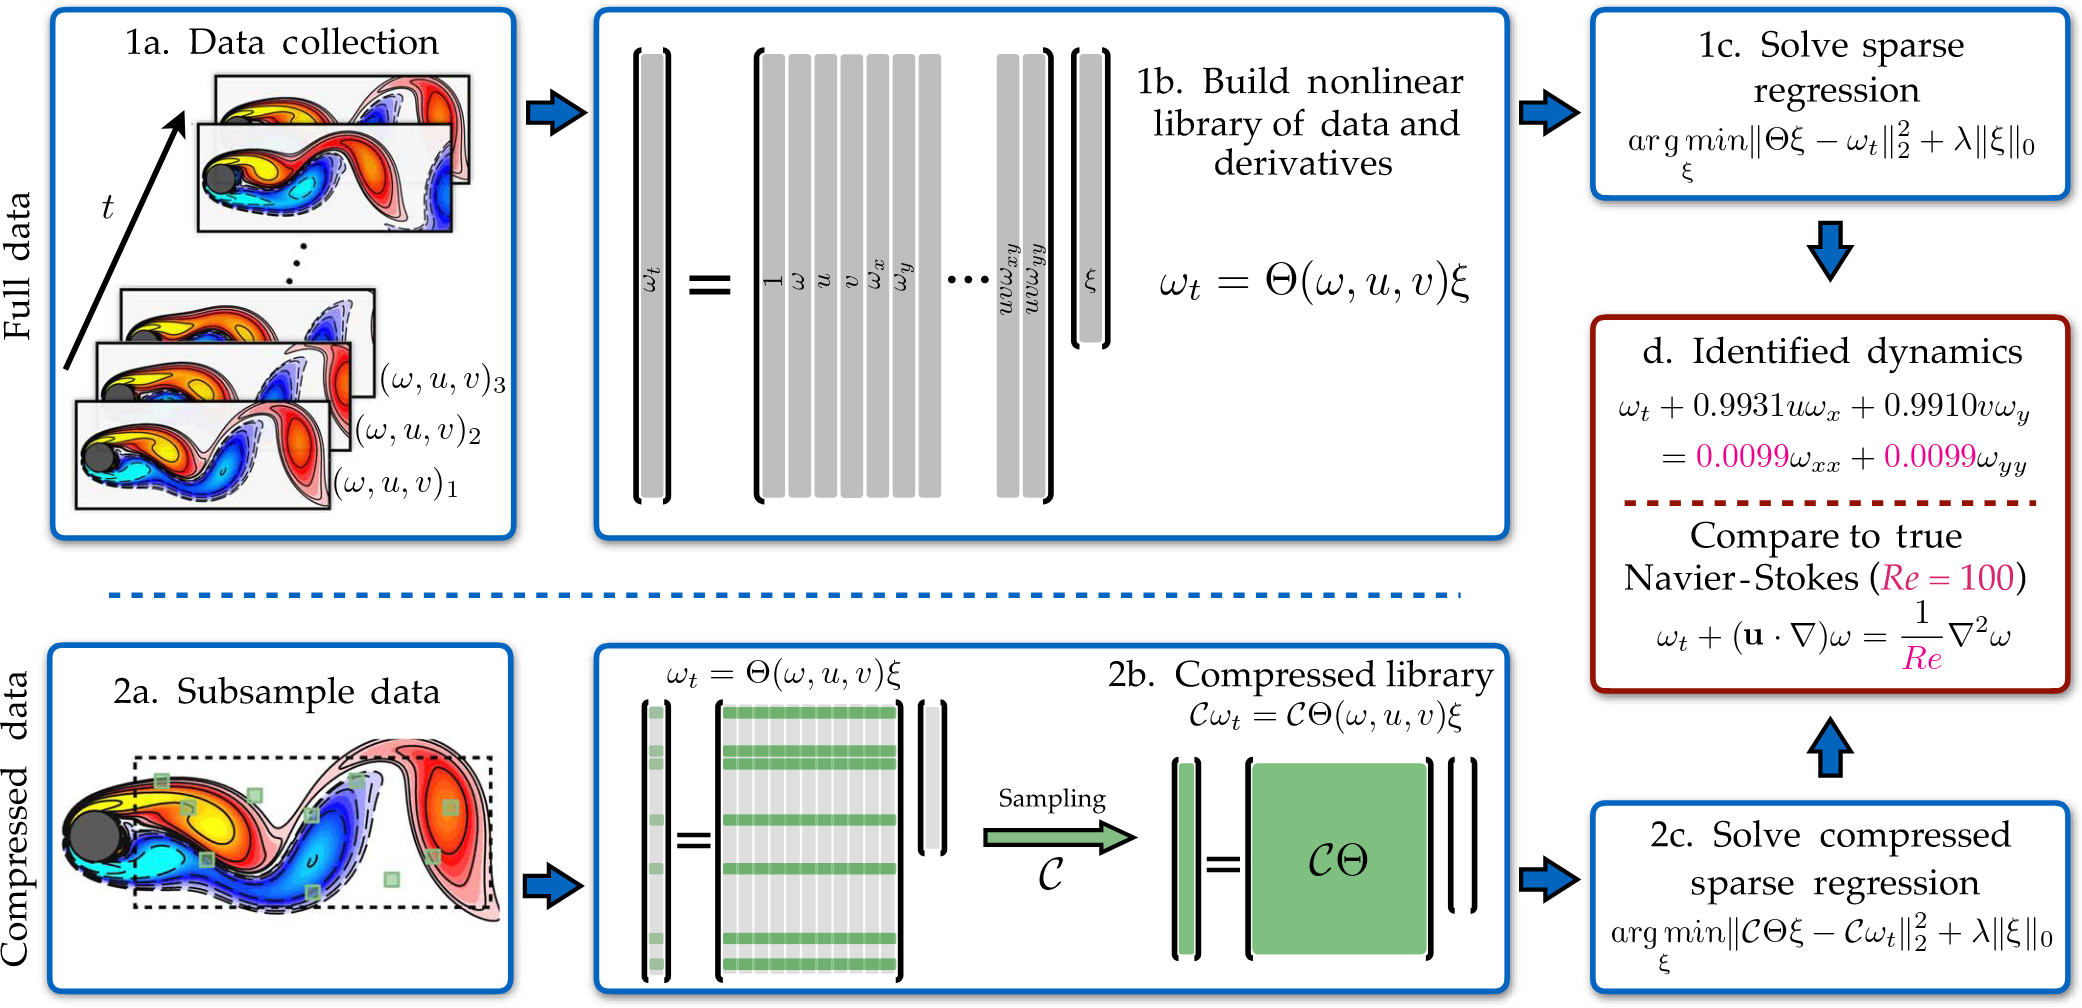
\includegraphics[width=\textwidth]{imgs/pde_find.png}
    \vfill
\end{frame}

\begin{frame}[plain, standout]
    \vfill
    \centering
    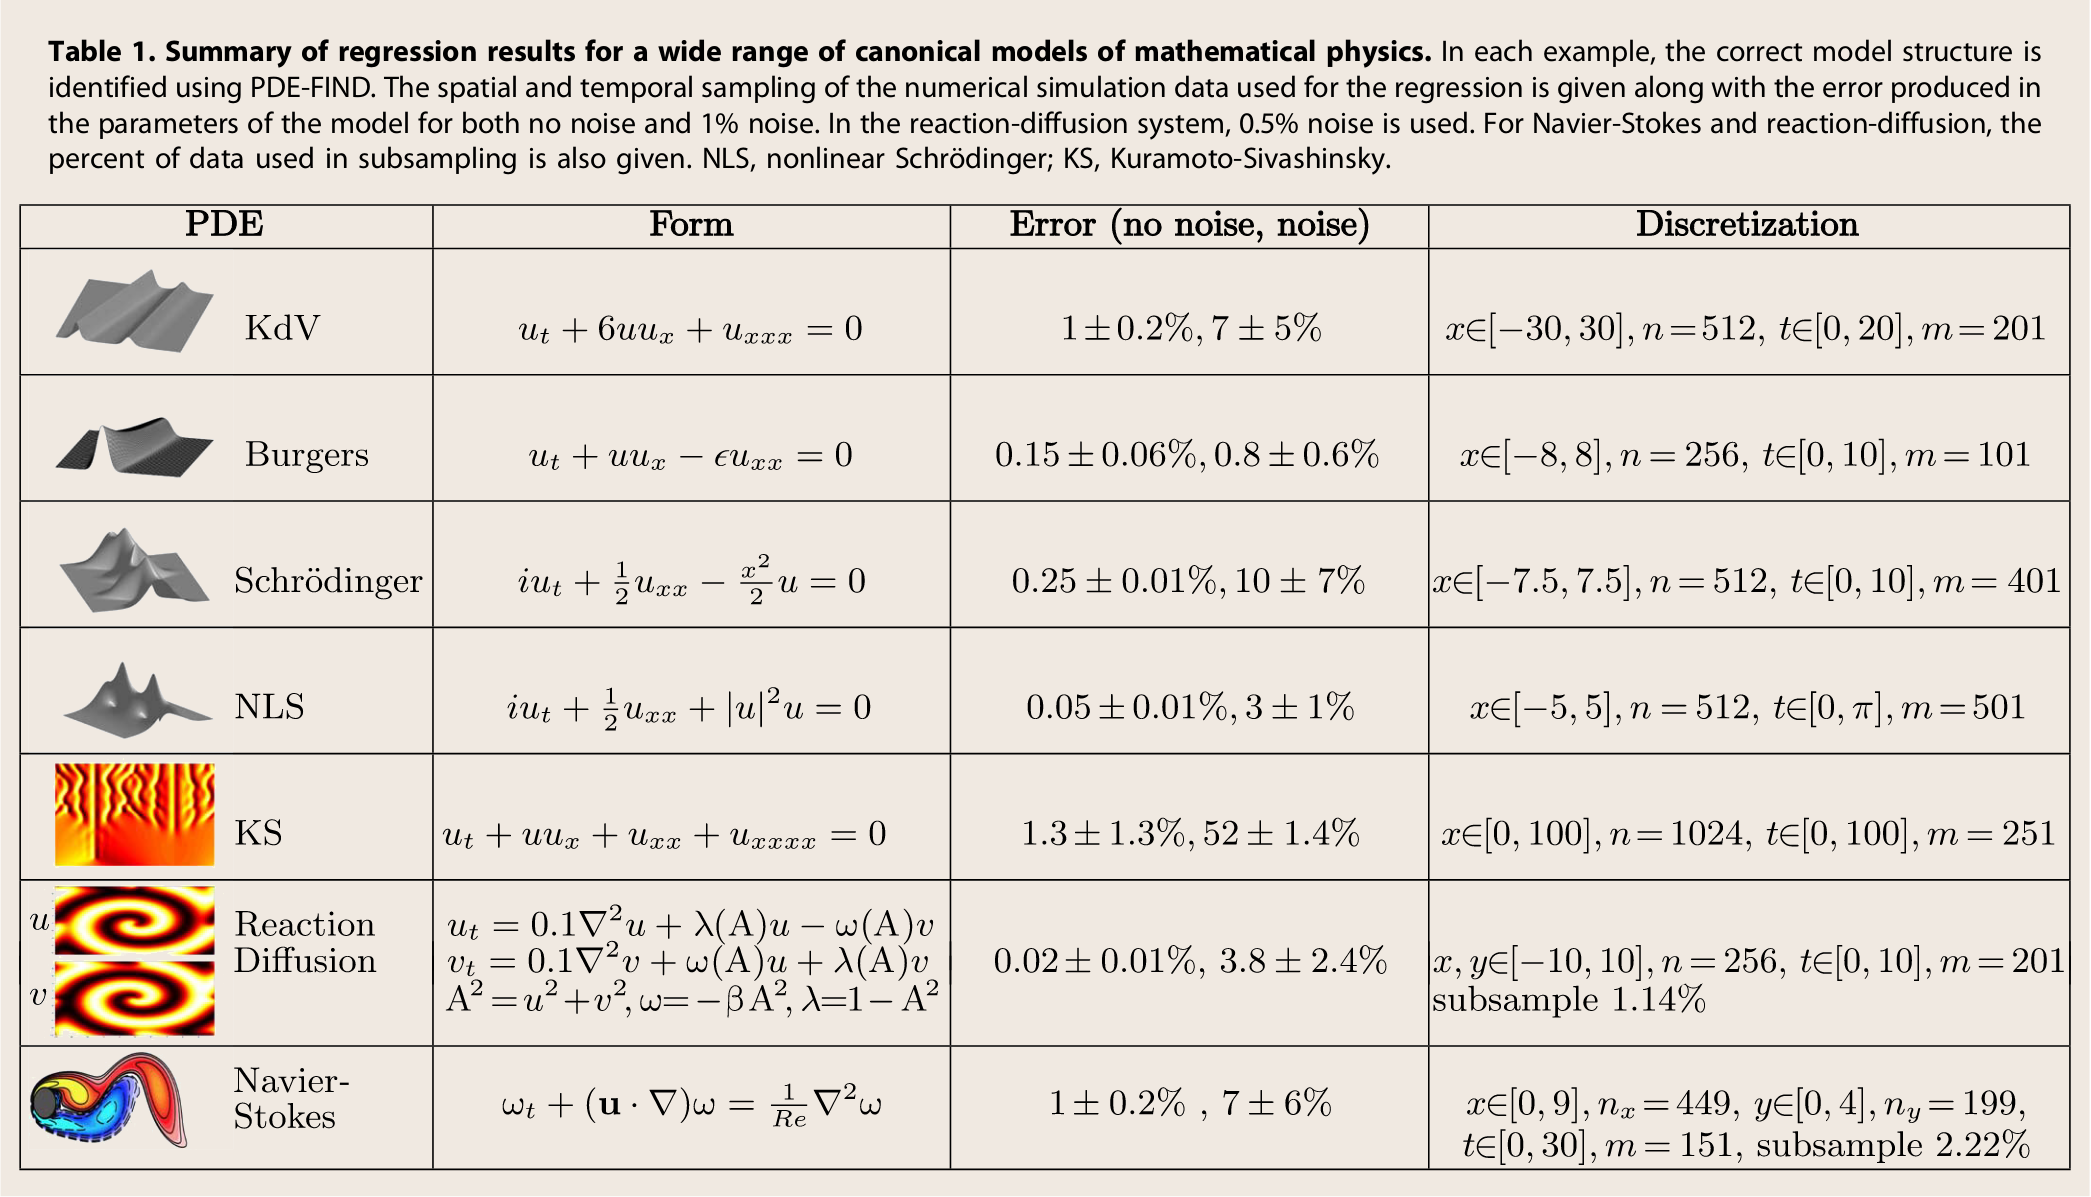
\includegraphics[width=\textwidth]{imgs/pde_find_results.png}
    \vfill
\end{frame}

\begin{frame}
    \vfill
    \begin{minipage}{.68\textwidth}
        \begin{itemize}
            \item Physical assumptions of \emph{smoothness}, \emph{locality} and \emph{symmetry} can be used to design an admissible dictionary.
            % \par\bigskip
            % \item Currently being used at CEA to infer a PDE from experimental PIV measurements of active turbulence.
            \par\bigskip
            \item Recent extension of incorporate assumptions of \emph{smoothness}, \emph{locality} and \emph{symmetry} to design \emph{a priori} a physically admissible dictionary.
        \end{itemize}
    \end{minipage}%
    \hfill
    \begin{minipage}{.28\textwidth}
        \centering
        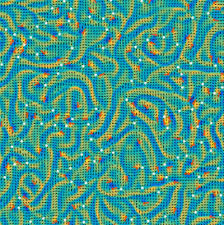
\includegraphics[width=\textwidth]{imgs/active_turbulence.jpeg}
    \end{minipage}
    \vfill
\end{frame}

\Section{SINDy for SDE}
\begin{frame}
    \frametitle{SINDy for Stochastic Diff. Eq.}
    \vfill
    \begin{minipage}{.48\textwidth}
        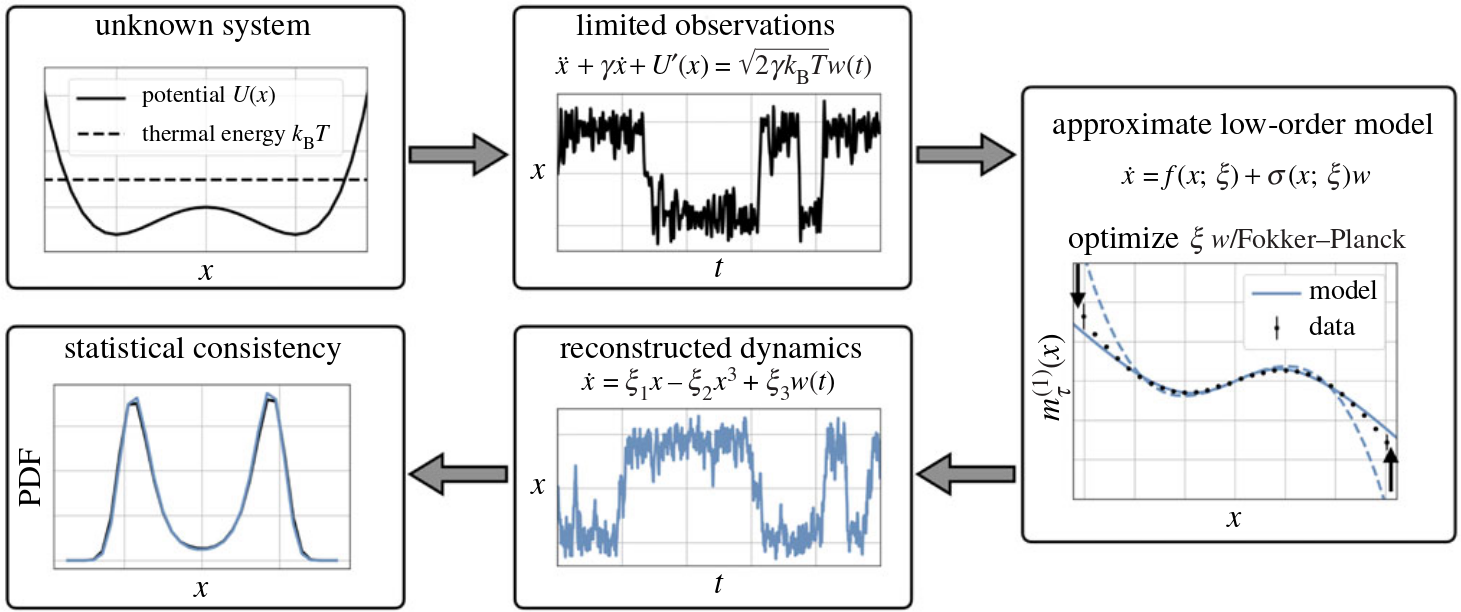
\includegraphics[width=\textwidth]{imgs/langevin_regression_one.png}
    \end{minipage}%
    \hfill
    \begin{minipage}{.48\textwidth}
        \begin{itemize}
            \item Many systems in physics can be described by \emph{Langevin equations}
            %
            \[
            \dot{x} = f(x) + \sigma(x) \eta.
            \]
            \item Identifying the drift and diffusion terms are is slightly more involved than vanilla SINDy.
        \end{itemize}
    \end{minipage}
    \vfill
\end{frame}

\begin{frame}
    \vfill
    \centering
    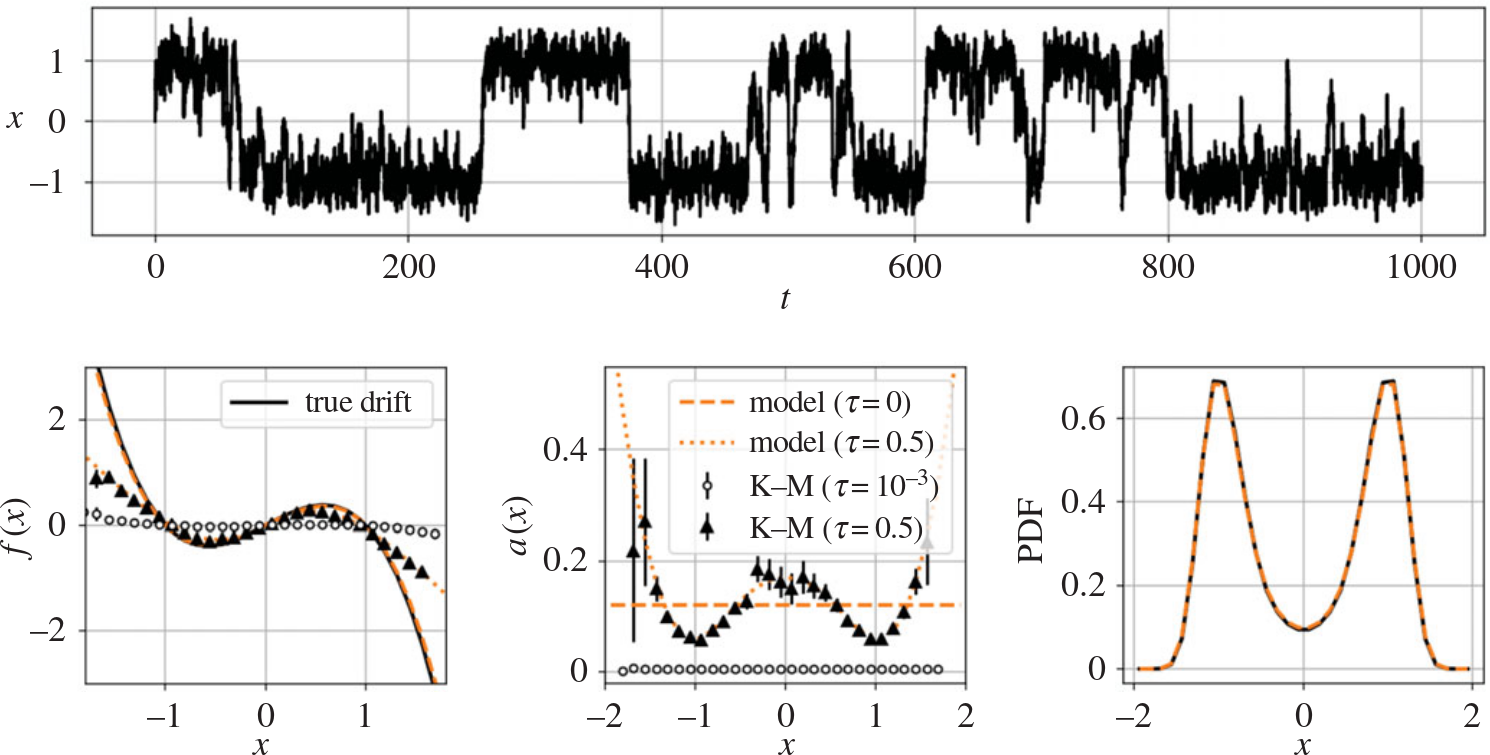
\includegraphics[width=\textwidth]{imgs/langevin_regression_three.png}
    \vfill
\end{frame}

\begin{frame}
    \vfill
    \centering
    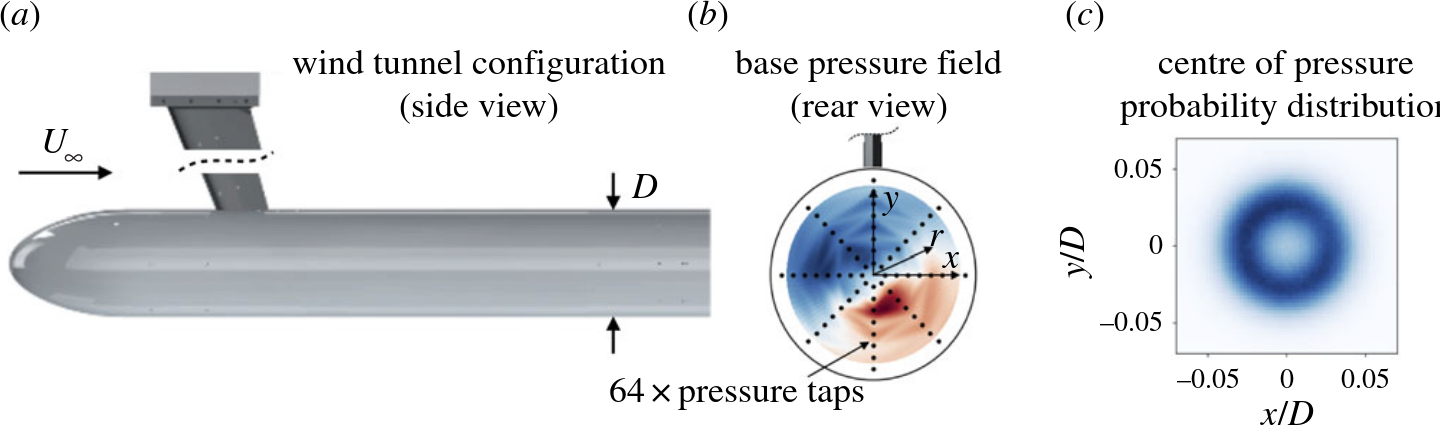
\includegraphics[width=\textwidth]{imgs/langevin_regression_four.png}
    \vfill
\end{frame}

\begin{frame}
    \vfill
    \centering
    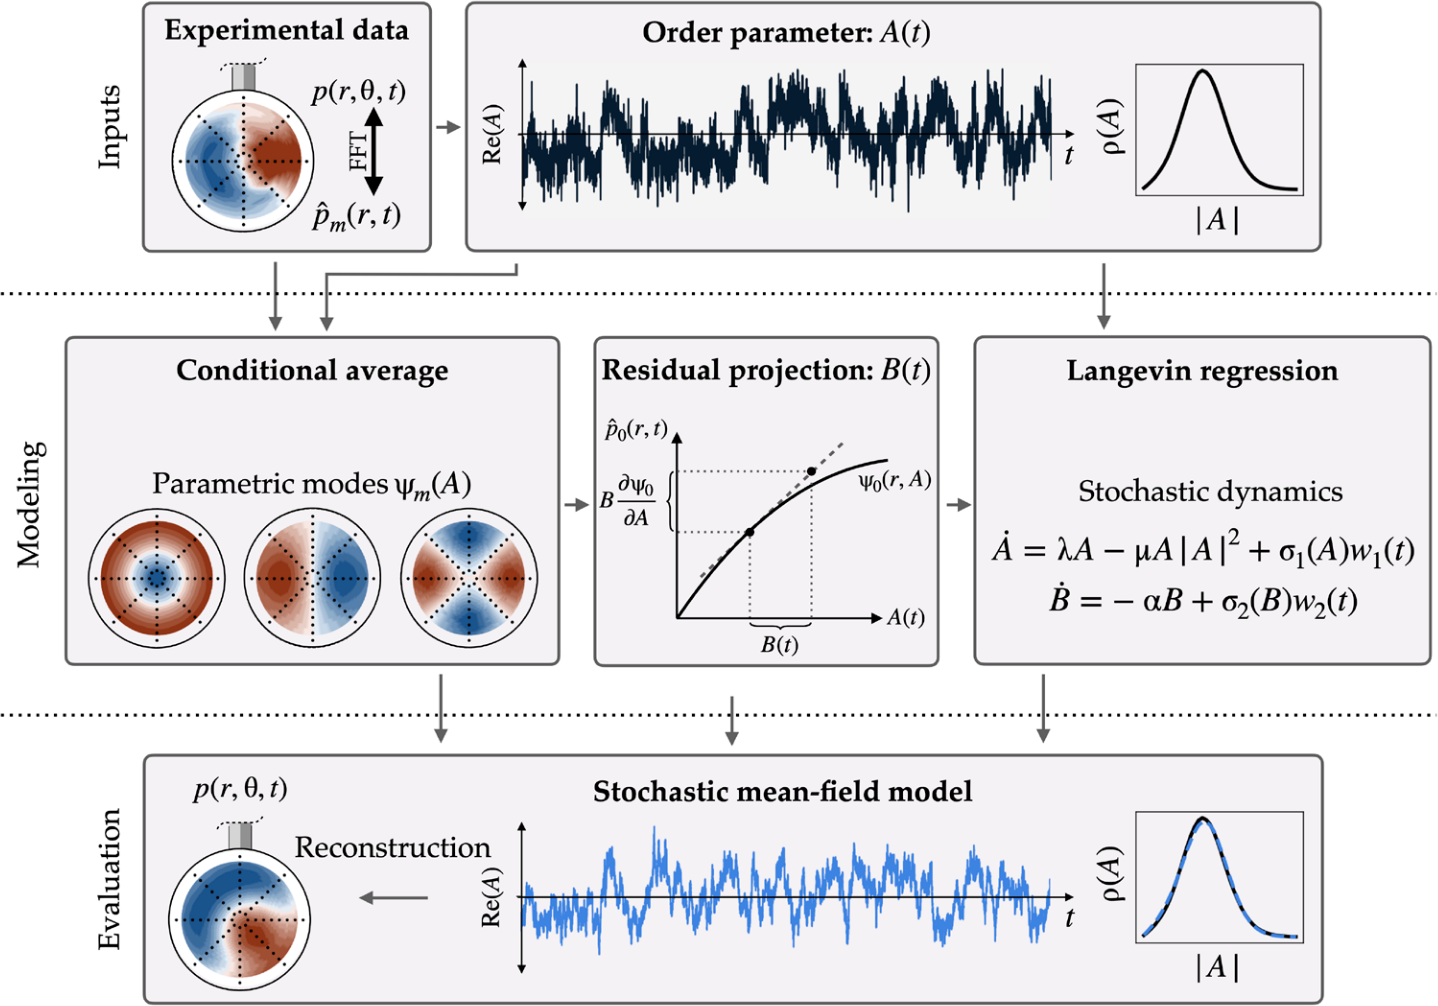
\includegraphics[height=.9\textheight]{imgs/langevin_regression_five.png}
    \vfill
\end{frame}

\Section{Reinf. Learning}
\begin{frame}
    \frametitle{SINDy for Reinf. Learning}
    \vfill
    \centering
    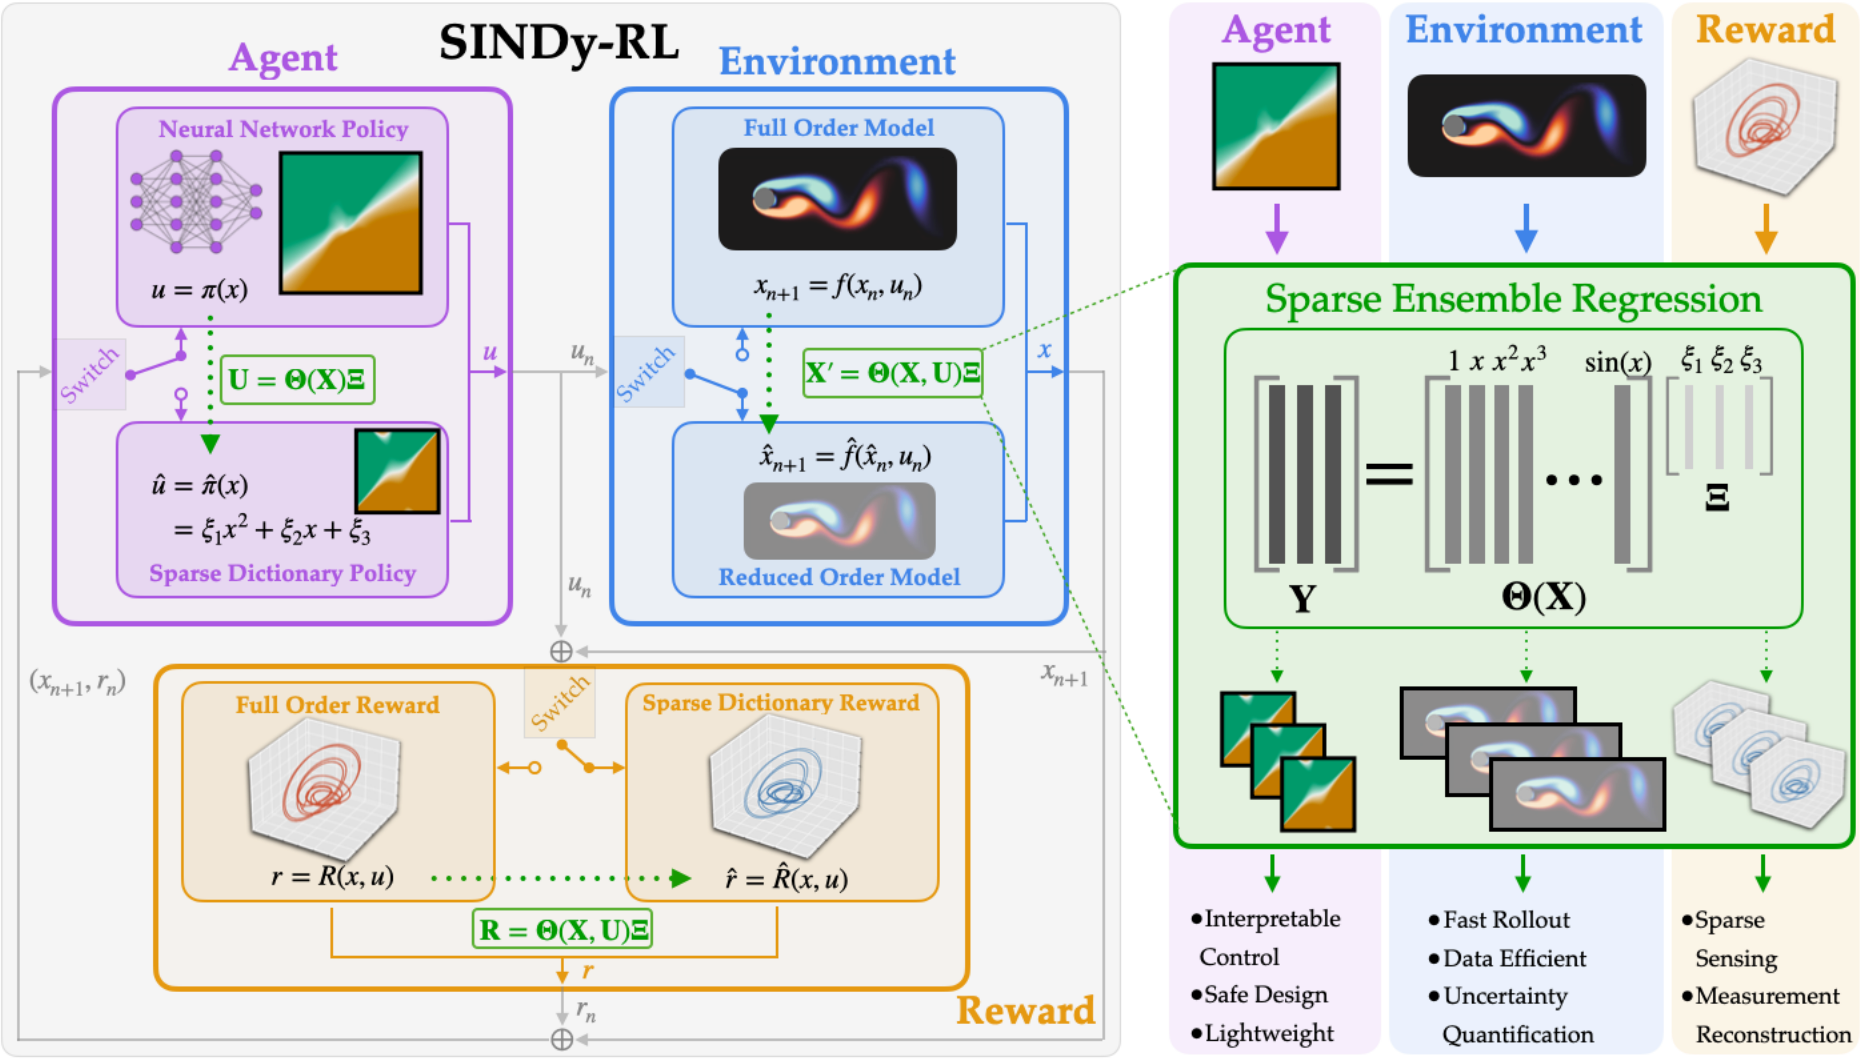
\includegraphics[width=.8\textwidth]{imgs/sindy_rl_one.png}
    \vfill
\end{frame}

\begin{frame}
    \vfill
    \centering
    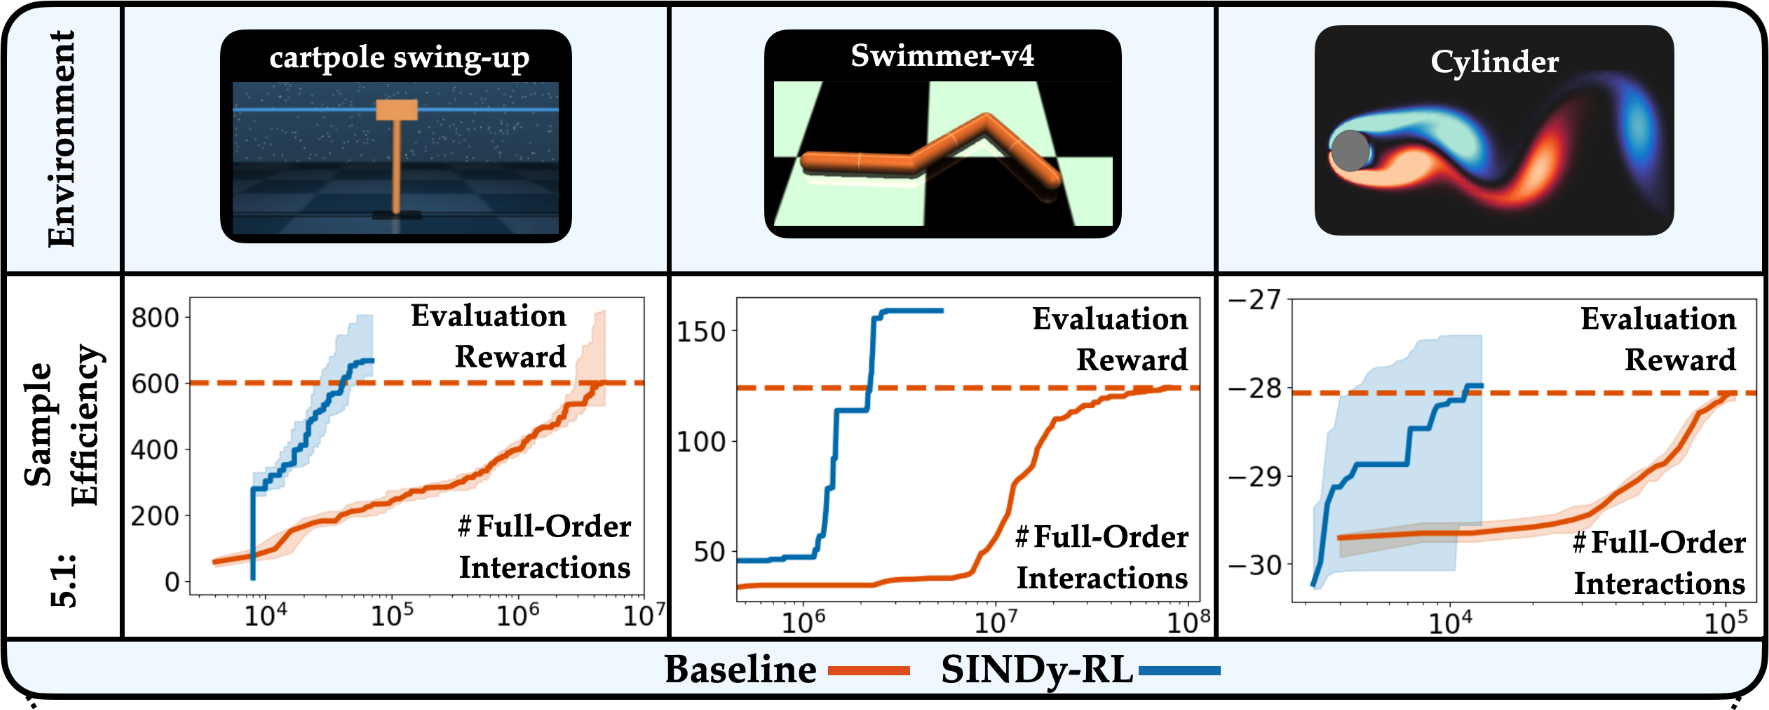
\includegraphics[width=\textwidth]{imgs/sindy_rl_two.png}
    \vfill
\end{frame}

% \Section{Control theory}
% \begin{frame}
%     \frametitle{SINDy for control systems}
% \end{frame}

\Section{Conclusion}
\begin{frame}[plain, standout]
    \vfill
    \begin{minipage}{.48\textwidth}
        \centering
        \Huge
        \textbf{Conclusion}
    \end{minipage}%
    \hfill
    \begin{minipage}{.48\textwidth}
    \end{minipage}
    \vfill
\end{frame}

\begin{frame}
    \frametitle{Conclusion}

    \vfill
    \begin{minipage}{.68\textwidth}
        \begin{itemize}
            \item Since 2015, \textbf{SINDy} has evolved into a mature ecosystem.
            \begin{itemize}
                \item Ordinary diff. eq., partial diff. eq., control systems, etc.
            \end{itemize}
            \par\bigskip
            \item Despite its versatility, \textbf{SINDy} is not a silver bullet.
            \begin{itemize}
                \item Requires quite a bit of domain expertise.
            \end{itemize}
        \end{itemize}
    \end{minipage}%
    \hfill
    \begin{minipage}{.28\textwidth}
        \centering
        
\includegraphics[width=\textwidth]{imgs/conclusion.png}
    \end{minipage}
    \vfill
\end{frame}

\begin{frame}
    \frametitle{PySINDy}
    \vfill
    \begin{minipage}{.38\textwidth}
        \centering
        \vspace{-2em}
        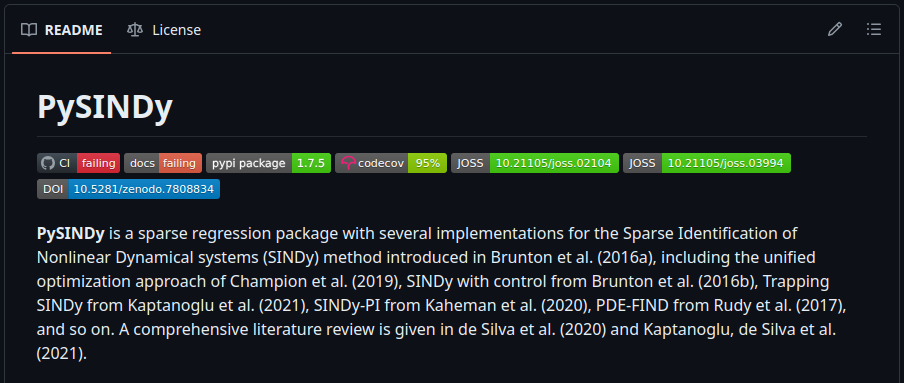
\includegraphics[width=\textwidth]{imgs/pysindy.png}
    \end{minipage}%
    \hfill
    \begin{minipage}{.58\textwidth}
        \begin{itemize}
            \item Open-source \texttt{Python} package with a simple and \texttt{scikit-learn} compatible API.
            \par\bigskip
            \item We're always on the look for new contributors!
            \begin{itemize}
                \item More computationally efficient algorithms.
                \item New/better variants of \textbf{SINDy}.
            \end{itemize}
        \end{itemize}
    \end{minipage}
    \vfill
\end{frame}

% \begin{frame}
%       \frametitle{A frame with title and subtitle}
%       \framesubtitle{Subtitle here}
%       Lorem ipsum dolor sit amet, consectetur adipiscing elit, sed do eiusmod tempor incididunt ut labore et dolore magna aliqua \par
%       Itemized list:
%       \begin{itemize}
%             \item Lorem ipsum
%             \item Dolor sit amet
%                   \begin{itemize}
%                         \item Consectetur
%                         \item Adipiscing elit
%                   \end{itemize}
%             \item Sed do eiusmod
%                   \begin{itemize}
%                         \item Tempor incididunt
%                               \begin{itemize}
%                                     \item Ut labore et dolore
%                                     \item Magna aliqua
%                               \end{itemize}
%                   \end{itemize}
%       \end{itemize}
% \end{frame}

% \begin{frame}
%       \frametitle{A frame with title only}
%       \begin{theorem}
%             \[e^{i\pi}+1=0\]
%             \begin{proof}
%                   \begin{equation*}
%                         e^{iz}=\cos{z}+i\sin{z}
%                   \end{equation*}
%                   \center{therefore}
%                   \begin{align*}
%                         e^{i\pi}+1 & \null=\cos\pi+i\sin\pi+1 \\
%                                    & \null=-1+i\times0+1      \\
%                                    & \null=0
%                   \end{align*}
%             \end{proof}
%       \end{theorem}
% \end{frame}

% \begin{frame}[bg=demo-arguelles.png]
%       \frametitle{A frame with background image}
%       You can still add title and subtitle. \par
%       You can also use a background in the title slide by setting: \\
%       \texttt{\textbackslash frame[plain,bg=demo-background.jpg]\{\textbackslash titlepage\}}
% \end{frame}

% \begin{frame}[plain]
%       \frametitle{A plain frame has no headline}
%       \begin{table}
%             \small
%             \begin{tabular}{rl}
%                   \ttfamily\textbackslash Alegreya              & \Alegreya Lorem ipsum dolor sit amet              \\
%                   \ttfamily\textbackslash AlegreyaMedium        & \AlegreyaMedium Lorem ipsum dolor sit amet        \\
%                   \ttfamily\textbackslash AlegreyaExtraBold     & \AlegreyaExtraBold Lorem ipsum dolor sit amet     \\
%                   \ttfamily\textbackslash AlegreyaBlack         & \AlegreyaBlack Lorem ipsum dolor sit amet         \\
%                   \ttfamily\textbackslash AlegreyaSansThin      & \AlegreyaSansThin Lorem ipsum dolor sit amet      \\
%                   \ttfamily\textbackslash AlegreyaSansLight     & \AlegreyaSansLight Lorem ipsum dolor sit amet     \\
%                   \ttfamily\textbackslash AlegreyaSans          & \AlegreyaSans Lorem ipsum dolor sit amet          \\
%                   \ttfamily\textbackslash AlegreyaSansMedium    & \AlegreyaSansMedium Lorem ipsum dolor sit amet    \\
%                   \ttfamily\textbackslash AlegreyaSansExtraBold & \AlegreyaSansExtraBold Lorem ipsum dolor sit amet \\
%                   \ttfamily\textbackslash AlegreyaSansBlack     & \AlegreyaSansBlack Lorem ipsum dolor sit amet
%             \end{tabular}
%       \end{table}
%       \vfill
%       \begin{alert}{Alert!}
%             A \textit{plain} frame does not show the progress bar but still appears in it unless the frame comes after \texttt{\textbackslash End}
%       \end{alert}
% \end{frame}

% \begin{frame}[standout]
%       \centering\large
%       A \textbf{\itshape\scshape standout} frame can be used to focus attention
% \end{frame}

\End

\begin{frame}
    This presentation wouldn't have been possible without many collaborators, including (but not limited to): 
    
    Steven Brunton, Bing Brunton, Nathan Kutz, Jared Callaham, Kathleen Champion, Brian da Silva, Alan Kaptanoglu, Kadierdan Kaheman, Urban Fasel, Sam Rudy, Zachary Nicolaou, Georgios Rigas, Nicholas Zolman and many others.
\end{frame}
\End

\begin{frame}[plain,standout]
    \vfill
    \begin{minipage}{.68\textwidth}
        {
            \Large
            \textbf{Thank you for your attention!}
        }
        \par\bigskip
        {
            Any questions?
        }
    \end{minipage}%
    \hfill
    \begin{minipage}{.28\textwidth}
        \centering
        \scalebox{4}{\faGithub} \par\bigskip
        \tiny
        \url{loiseaujc.github.io}
    \end{minipage}
    \vfill
\end{frame}

\end{document}
